\documentclass[a4paper, 11pt,notoc]{article}
\pdfoutput=1
\usepackage{jcappub}
\usepackage{graphicx}
\usepackage{booktabs}
\usepackage{verbatim}
\usepackage{caption}
\usepackage{xspace}
\usepackage{hyperref}
\usepackage{multirow}
\usepackage{placeins}

%\usepackage[skip=0cm,list=true,labelfont=it]{subcaption}
\usepackage{subcaption}
%\usepackage[sorting=none,backend=biber]{biblatex}

\usepackage{units}
\usepackage{draftwatermark}
\SetWatermarkText{LHC DM WG DRAFT}
\SetWatermarkLightness{0.9}
\SetWatermarkScale{3.0}
\newcommand{\bra}[1]{\langle #1|}
\newcommand{\ket}[1]{|#1\rangle}
\newcommand{\sigv}{\ensuremath{\langle \sigma v_{\rm{rel}} \rangle}\xspace}
\newcommand{\MET}{\ensuremath{E_T^\mathrm{miss}}\xspace}
\newcommand{\met}{\MET}
\newcommand{\MT}{\ensuremath{M_{T}}\xspace}
%\newcommand{\MET}{\ensuremath{\slashed{E}_T}\xspace}
%\newcommand{\met}{\ensuremath{\slashed{E}_T}\xspace}
\newcommand{\mDM}{\ensuremath{M_{\chi}}\xspace}
\newcommand{\mmed}{\ensuremath{M_{\rm{med}}}\xspace}
\newcommand{\mMed}{\ensuremath{M_{\rm{med}}}\xspace}
\newcommand{\mZ}{\ensuremath{M_{\rm{Z}}}\xspace}
\newcommand{\gDM}{\ensuremath{g_{\rm{DM}}}\xspace}
\newcommand{\gq}{\ensuremath{g_q}\xspace}
\newcommand{\gSM}{\gq}
\newcommand{\gdm}{\gDM}
\newcommand{\ifb}{\ensuremath{\rm{fb}^{-1}}\xspace}
\newcommand{\mA}{\ensuremath{M_{A}}\xspace}
\newcommand{\ma}{\ensuremath{M_{a}}\xspace}
\newcommand{\mH}{\ensuremath{M_{H}}\xspace}
\newcommand{\mHc}{\ensuremath{M_{H^{\pm}}}\xspace}
\newcommand{\sinp}{\ensuremath{\sin\theta}\xspace}
\newcommand{\cosp}{\ensuremath{\cos\theta}\xspace}
\newcommand{\sinbma}{\ensuremath{\sin(\beta - \alpha)}\xspace}
\newcommand{\tanb}{\ensuremath{\tan\beta}\xspace}
\newcommand{\lap}[1]{\lambda_{P#1}} % can use like \lap1 , \lap2
\newcommand{\lam}[1]{\lambda_{#1}} % can use like \lam3
\newcommand{\mh}{\ensuremath{M_{h}}\xspace}
\newcommand{\mt}{\ensuremath{M_{t}}\xspace}
\newcommand{\GamA}{\ensuremath{\Gamma_{A}}\xspace}
\newcommand{\Uli}{\color{red}}
\definecolor{cerulean}{RGB}{44,150,207}
\newcommand{\ATLASComments}{\color{cerulean}}
\newcommand{\dmsimp}{\textsc{DMsimp}\xspace}
\newcommand{\maddm}{\textsc{MadDM}\xspace}
\newcommand{\hdm}{\ensuremath{h+\textrm{DM}}\xspace}
\newcommand{\monoh}{\ensuremath{h+\MET}\xspace}
\newcommand{\monohbb}{\ensuremath{h(bb)+\MET}\xspace}
\newcommand{\monoz}{\ensuremath{Z+\MET}\xspace}
\newcommand{\monozll}{\ensuremath{Z(\ell\ell)+\MET}\xspace}
\newcommand{\monozhad}{\ensuremath{Z(\textrm{had})+\MET}\xspace}
\newcommand{\mg}{\textsc{MadGraph~5}\xspace}
\newcommand{\sens}{\mathcal{S}\xspace}
\newcommand{\senstot}{\mathcal{S}_\textrm{tot}\xspace}
\newcommand{\GeV}{\textrm{GeV}\xspace}
\newcommand{\gev}{\GeV\xspace}
\newcommand{\hdma}{\ensuremath{\textrm{2HDM+a}}\xspace}

\newcommand{\lp}{\ensuremath{l^{+}}\xspace}
\newcommand{\lm}{\ensuremath{l^{-}}\xspace}
\newcommand{\pt}{\ensuremath{p_{T}}\xspace}

\newcommand{\ttbar}{\ensuremath{\bar{t}t}}
\newcommand{\bbbar}{\ensuremath{\bar{b}b}}
%\newcommand*{\TeV}{\ensuremath{\text{Te\kern -0.1em V}}}
%\newcommand*{\GeV}{\ensuremath{\text{Ge\kern -0.1em V}}}
%\newcommand{\pt}{\ensuremath{p_{\mathrm T}}}
%\newcommand{\met}{\ensuremath{E_{\mathrm T}^{\mathrm miss}}}


%DIF PREAMBLE EXTENSION ADDED BY LATEXDIFF
%DIF UNDERLINE PREAMBLE %DIF PREAMBLE
\RequirePackage[normalem]{ulem} %DIF PREAMBLE
\RequirePackage{color}\definecolor{RED}{rgb}{1,0,0}\definecolor{BLUE}{rgb}{0,0,1} %DIF PREAMBLE
\providecommand{\DIFadd}[1]{{\protect\color{blue}\uwave{#1}}} %DIF PREAMBLE
\providecommand{\DIFdel}[1]{{\protect\color{red}\sout{#1}}}                      %DIF PREAMBLE
%DIF SAFE PREAMBLE %DIF PREAMBLE
\providecommand{\DIFaddbegin}{} %DIF PREAMBLE
\providecommand{\DIFaddend}{} %DIF PREAMBLE
\providecommand{\DIFdelbegin}{} %DIF PREAMBLE
\providecommand{\DIFdelend}{} %DIF PREAMBLE
%DIF FLOATSAFE PREAMBLE %DIF PREAMBLE
\providecommand{\DIFaddFL}[1]{\DIFadd{#1}} %DIF PREAMBLE
\providecommand{\DIFdelFL}[1]{\DIFdel{#1}} %DIF PREAMBLE
\providecommand{\DIFaddbeginFL}{} %DIF PREAMBLE
\providecommand{\DIFaddendFL}{} %DIF PREAMBLE
\providecommand{\DIFdelbeginFL}{} %DIF PREAMBLE
\providecommand{\DIFdelendFL}{} %DIF PREAMBLE
%DIF END PREAMBLE EXTENSION ADDED BY LATEXDIFF


\begin{document}
\title{\begin{boldmath} \huge Dark Matter Working Group recommendation for Two Higgs Doublet Model (draft title) \vspace{7mm} \end{boldmath}}

%%%%%%

\affiliation[*]{DMWG organizers}

%\author[1,]{Andreas~Albert,}
%\affiliation[1]{III. Physikalisches Institut A, RWTH Aachen University, Aachen, Germany}

%\author[2]{Mihailo Backovi\'c,}
%\affiliation[2]{Center for Cosmology, Particle Physics and Phenomenology - CP3, Universite Catholique de Louvain, Louvain-la-neuve, Belgium}

\author[]{Authorlist to be compiled; }

\author[3,*]{Antonio~Boveia,}
\affiliation[3]{Ohio State University, 191 W. Woodruff Avenue
Columbus, OH 43210}
\emailAdd{antonio.boveia@cern.ch}

%\author[4,*]{Oliver~Buchmueller,}
%\affiliation[4]{High Energy Physics Group, Blackett Laboratory, Imperial College, Prince Consort Road, London, SW7 2AZ, United Kingdom}
%\emailAdd{oliver.buchmueller@cern.ch}

%\author[5,*]{Giorgio Busoni,} 
%\affiliation[5]{ARC Centre of Excellence for Particle Physics at the Terascale, School of Physics, University of Melbourne, 3010, Australia}

%\author[6,7]{Albert De~Roeck,}
%\affiliation[6]{Antwerp University, BÐ2610 Wilrijk, Belgium. }
%\affiliation[7]{CERN, EP Department, CH-1211 Geneva 23, Switzerland}

\author[8,*]{Caterina~Doglioni,}
\affiliation[8]{Fysiska institutionen, Lunds universitet, Lund, Sweden}
\emailAdd{caterina.doglioni@cern.ch}

%\author[9,*]{Tristan~DuPree,}
%\affiliation[9]{Nikhef, Science Park 105, NL-1098 XG Amsterdam, The Netherlands}


%\author[10,*]{Malcolm Fairbairn,}
%\affiliation[10]{Physics, King's College London, Strand, London, WC2R 2LS, UK}

%\author[11]{\\ Marie-Helene Genest,}
%\affiliation[11]{Laboratoire de Physique Subatomique et de Cosmologie, Université Grenoble-Alpes, \\ CNRS/IN2P3, 53 rue des Martyrs, 38026 Grenoble Cedex, France}

%\author[12]{Stefania Gori,}
%\affiliation[12]{Department of Physics, University of Cincinnati, Cincinnati, Ohio 45221, USA}

%\author[13]{Giuliano~Gustavino,}
%\affiliation[13]{Universita' di Roma Sapienza, Piazza Aldo Moro, 2, 00185 Roma, Italy e INFN}

\author[14,*]{Kristian~Hahn,}
\affiliation[14]{Department of Physics and Astronomy, Northwestern University, Evanston, Illinois 60208, USA}
\emailAdd{kristian.hahn@cern.ch}

\author[15,16,*]{Ulrich~Haisch,}
\affiliation[15]{Rudolf Peierls Centre for Theoretical Physics, University of Oxford, Oxford, OX1 3PN, United Kingdom}
\affiliation[16]{CERN, TH Department, CH-1211 Geneva 23, Switzerland}
\emailAdd{ulrich.haisch@physics.ox.ac.uk}


%\author[7]{Philip~C.~Harris,} 

%\author[17]{Dan~Hayden,}
%\affiliation[17]{Michigan State University, 220 Trowbridge Rd, East Lansing, MI 48824,
%USA}

%\author[18]{Valerio~Ippolito,} 
%\affiliation[18]{Laboratory for Particle Physics and Cosmology, Harvard University, USA}

%\author[8]{Isabelle~John,}

%\author[19,*]{Felix~Kahlhoefer,}
%\affiliation[19]{DESY, Notkestra\ss e 85, D-22607 Hamburg, Germany}

%\author[20]{Suchita~Kulkarni,}
%\affiliation[20]{Institut f\"ur Hochenergiephysik, \"Osterreichische Akademie der Wissenschaften, \\ Nikolsdorfer Gasse 18, 1050 Wien, Austria}

%\author[21]{Greg Landsberg,}
%\affiliation[21]{Brown University, Dept. of Physics, 182 Hope St, Providence, RI 02912, USA.}

\author[22]{Steven Lowette,}
\affiliation[22]{Physics Department, Vrije Universieit Brussel, Brussels, Belgium}

%\author[11]{Kentarou~Mawatari,}

%\author[23]{Antonio Riotto,}
%\affiliation[23]{Departement de Physique Theorique (DPT) Geneva Cosmology and Astroparticle Group and Centre for Astroparticle Physics  (CAP), 24 quai Ernest Ansermet
%CH-1211 Geneve}

%\author[24]{William~Shepherd,}
%\affiliation[24]{Institut f\"ur Physik, Johannes-Gutenberg-Universit\"at Mainz, Staudingerweg 7, D-55128 Mainz, Germany}

\author[25,*]{Tim~M.P.~Tait,}
\affiliation[25]{Department of Physics and Astronomy, University of California, Irvine, California 92697, USA}
\emailAdd{ttait@uci.edu}

%\author[3]{Emma Tolley,}

%\author[10,*]{\\ Patrick Tunney,}

%\author[26,*]{Bryan~Zaldivar,}
%\affiliation[26]{Laboratoire de Physique Theorique d'Annecy-le-Vieux (LAPTH) 9 Chemin de Bellevue, B.P. 110, F-74941 Annecy-le-Vieux, CEDEX, France}

%\author[24]{Markus~Zinser}


\hfill CERN-LPCC-2017-XX


\abstract{
Draft abstract.}
\maketitle


%%%%%%%%%%%%%%%%
\section{Introduction}
\paragraph{Reasoning behind this effort}

\begin{itemize}
\item Simplified models only one signature at a time, sometimes not
gauge invariant
\item One step beyond this: less-simplified models

\item Compare and confront different search sensitivity

\item Combinations among different signatures

\item Find new kinematic regimes / improve searches by exploring
different signatures

\item Still keeping the choice of model generic enough that this is reusable
for theorists

\end{itemize}

\paragraph{Reasoning behind this effort}

\begin{itemize}

\item Reasoning behind the choice of model

\item Highlights more than one signature at a time, depending on
parameters

\item Leaves room for new unexplored kinematic signatures within
existing searches (left for future work)

\item Complete enough, still simplified so that one can choose grid
planes

\item Existing theory effort (HXSWG)
\end{itemize}

We investigate in detail the kinematics of three experimental signatures that are sensitive to this model: 

\begin{itemize}
\item the Higgs+\MET signature, where the \MET is produced by the decay of the pseudoscalar that couples to dark matter and the Higgs is produced either in association with this pseudoscalar or as a product of the decay of the second pseudoscalar; 

\item the Z+\MET signature, where the \MET is produced by the decay of the pseudoscalar that couples to dark matter and the Z boson is either produced in association with this pseudoscalar or radiated by the heavy Higgs boson; 

\item the $t\bar{t}$+\MET signature, where pseudoscalar that couples to dark matter is produced in association with a $t\bar{t}$ pair or radiated by one of the top quarks. 

\item 
\end{itemize}

The sensitivity of searches for this model in those signatures surpasses that of the jet+\MET searches, providing a motivation to explore their parameter space beyond the $s-$channel simplified models in~\cite{Abercrombie:2015wmb}. 

Moreover, we identify a number of other signatures that have sensitivity to this model and can be studied in the future, such as ...

\section{The model}
\paragraph{Description of the model}

\begin{itemize}

\item Citations: \cite{Bauer:2017ota, Bell:2016ekl, Ipek:2014gua, No:2015xqa, Goncalves:2016iyg}

\item Particles, masses, couplings, mixing angles

\end{itemize}

\paragraph{Comparison with existing models}

How does the model compare with other 2HDMs/scalar models (with and without DM). 

\begin{itemize}
    \item Scalar to SSM to 2HDM evolution
    \item Other models:
    \begin{itemize}
        \item S. Ipek, D. McKeen, A. Nelson, \cite{Ipek:2014gua}
        \item Bell, Busoni, Sanderson, \cite{Bell:2016ekl}
        \item No, Goncalves, Machado, \cite{No:2015xqa, Goncalves:2016iyg}
        \item Higgs Cross-section Working Group
    \end{itemize}
\end{itemize}


\section{Model parameters}
\begin{itemize}
    \item Motivate the choice of parameters in~\cite{Bauer:2017ota}
    
    
    \item Vacuum stability study: fix lambda parameters to 3
    
    For extension of the Higgs sector (and in general for scalar extensions of the Standard Model) one needs to worry about 
    boundedness from below of the scalar potential, as well as absolute stability of the electroweak minimum\footnote{We remark 
    here that implications from all indirect constraints - be it flavour, electroweak precision constraints or stability 
    requirements -  should be treated as preferred parameter space in a simplified model framework. It would contradict the idea of simplified
models were these constraints taken at face value.}.  

    Regarding boundedness from below of the scalar potential in the present 2HDM + S model, we stress that provided that 
    $\lambda_{P1}, \, \lambda_{P2} > 0$ in
    %
    \begin{eqnarray}
     V_{\mathrm{P}} = \frac{1}{2} m_{P}^2 P^2 + \kappa\, (i \,P\, H_1^{\dagger}H_2 + \mathrm{h.c.}) \nonumber \\
            + \lambda_{P1} \,P^2\, \left|H_1\right|^2 + \lambda_{P2} \,P^2 \,\left|H_2\right|^2 \, ,\nonumber
    \end{eqnarray}
    %
    the study of boundedness from below at tree-level reduces to the corresponding study in the 2HDM. The boundedness from below conditions 
    in this case are well-known~\cite{Gunion:2002zf}:
    %
    \begin{equation}
    \label{stability2HDM}
     \lambda_1 > 0\,, \,\,\, \lambda_2 > 0\,, \,\,\, \lambda_3 > - \sqrt{\lambda_1 \lambda_2} \,, \,\,\, \lambda_3 + \lambda_4 - |\lambda_5| > - \sqrt{\lambda_1 \lambda_2} 
    \end{equation}
    %
    and can be inferred from analyzing the scalar potential at large field values $H_1,\,H_2 \gg v$. For $m_{H^{\pm}} = m_{H_0}$, the first two conditions 
    in~\eqref{stability2HDM} may be simply written as
    %
    \begin{equation}
     \frac{m_h^2}{v^2} (1-t_{\beta}^{2}) + \lambda_3 \, t_{\beta}^{2} > 0\,, \quad\,\, \frac{m_h^2}{v^2} (1-t_{\beta}^{-2}) + \lambda_3 \, t_{\beta}^{-2} > 0
     \end{equation}
    %
    which result in the requirement $\lambda_3 > m_h^2/v^2 = 0.258$. In figure~\ref{Fig_Stability} we show the regions of parameter space in the 
    ($m_a,\, m_{H_0}$) (left) and ($s_{\theta},\, m_a$) (right) planes for which the tree-level boundedness from below conditions~\ref{stability2HDM}
    are satisfied, assuming $m_{H^{\pm}} = m_{H_0} = m_{A_0}$.
    %
    %
    \begin{figure}[h!]
\begin{center}
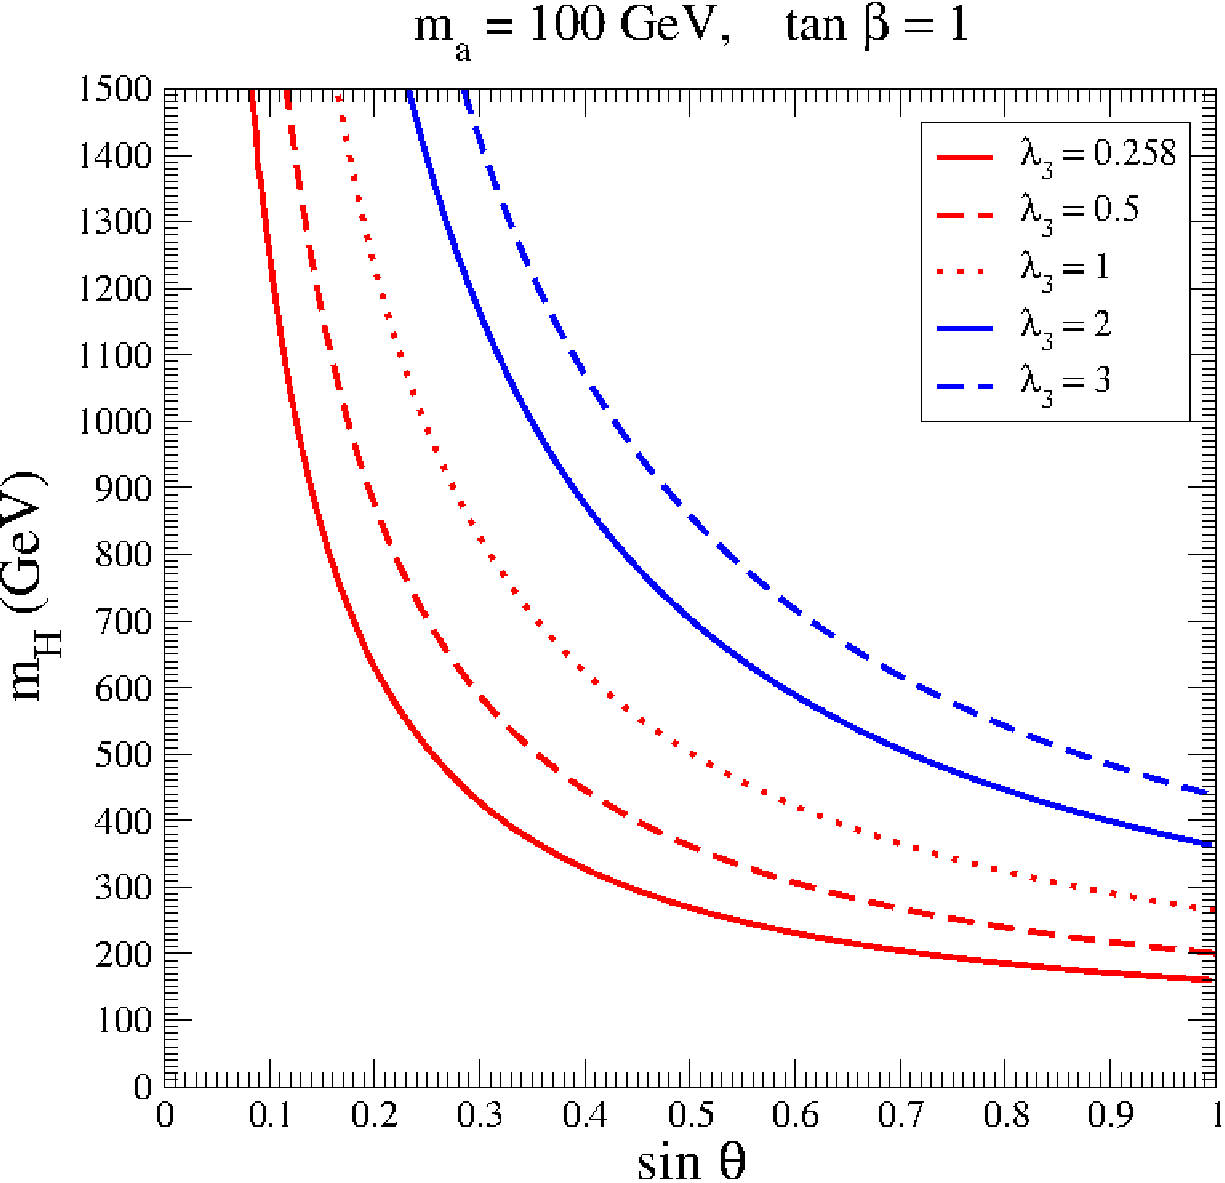
\includegraphics[width=0.485\textwidth]{texinputs/03_theoparameters/Figs/Plot_Eq.pdf}
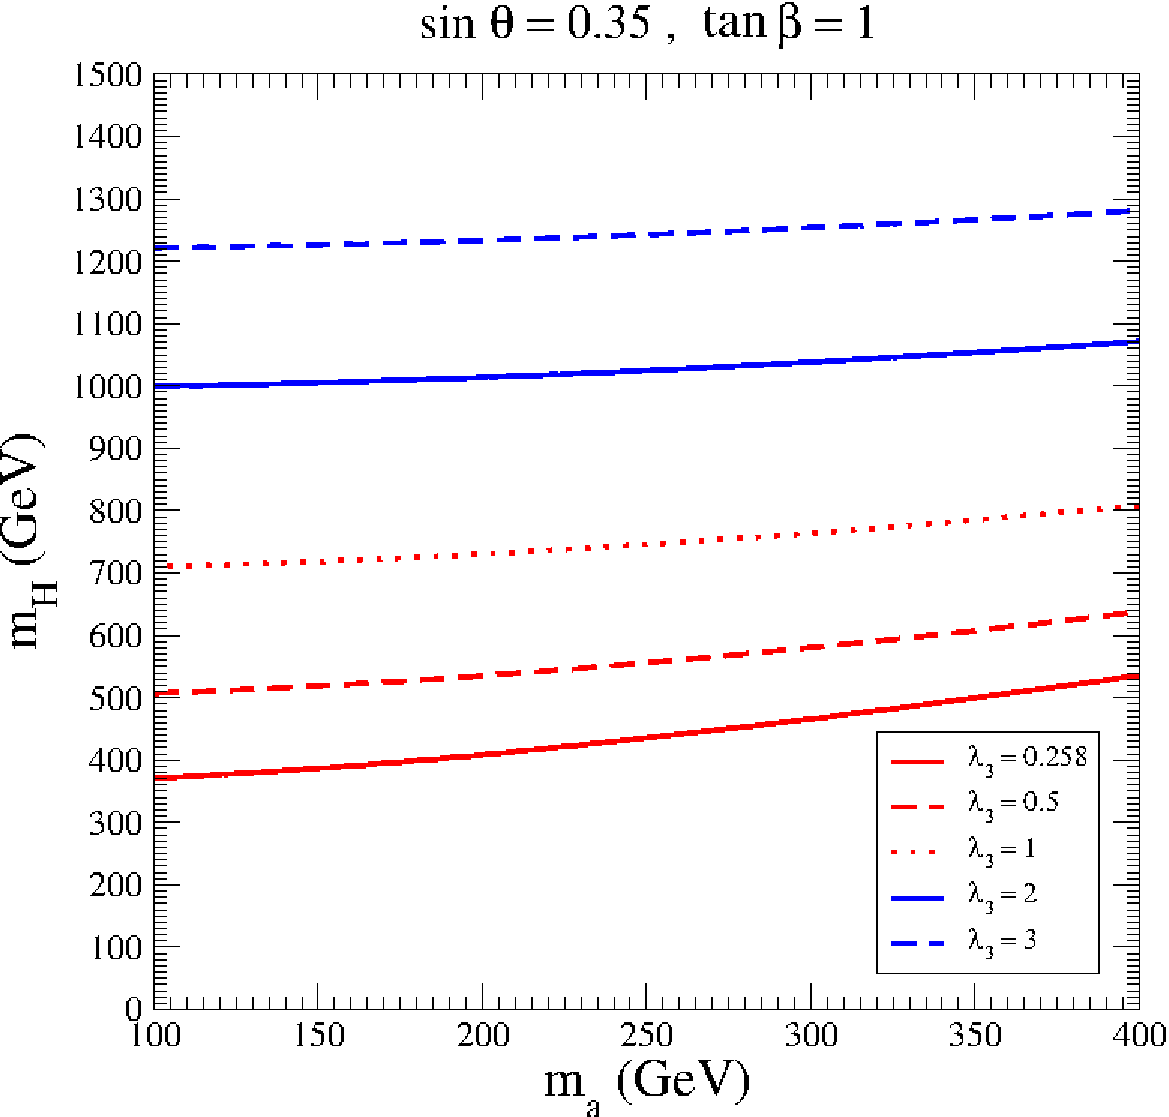
\includegraphics[width=0.485\textwidth]{texinputs/03_theoparameters/Figs/Plot_ma.pdf}
\caption{\small Regions of parameter space in the 
    ($m_a,\, m_{H_0}$) (left) and ($s_{\theta},\, m_a$) (right) planes for which the tree-level boundedness from below conditions~\ref{stability2HDM}
    are satisfied, assuming $m_{H^{\pm}} = m_{H_0} = m_{A_0}$. 
}
\label{Fig_Stability}
\end{center}

\vspace{-2mm}

\end{figure}
    %
    %
    
    Figure~\ref{Fig_Stability} shows that the region satisfying the tree-level boundedness from below conditions increases as $\lambda_3$ increases. At the same time, 
    the choice $\lambda_3 = \lambda_{P1} = \lambda_{P2}$ which we adopt in the present analysis allows the increase in $\lambda_3$  not to affect the mono-Higgs sensitivity
    via a change in the coupling $g_{aAh}$
    %
    \begin{eqnarray}
     g_{aAh} &=& \frac{c_{\theta} \,s_{\theta}}{m_{H} \,v} \left[m_h^2 + m_H^2 -m_a^2 - 2 
     (\lambda_3 - \lambda_{P1} c_{\beta}^2 - \lambda_{P2} s_{\beta}^2) v^2 \right] \nonumber \\
      &=& \frac{c_{\theta} \,s_{\theta}}{m_{H} \,v} \left[m_h^2 + m_H^2 -m_a^2 \right] 
    \end{eqnarray}
    %
    We then fix the value $\lambda_3 = 3$ as benchmark for the rest of our analysis. 
    
    \vspace{3mm}
    
    A few comments are in order. 
    
    \begin{itemize}
     \item The choice of $\lambda_3$, motivated by boundedness from below conditions, while not affecting the mono-Higgs sensitivity 
    if $\lambda_3 = \lambda_{P1} = \lambda_{P2}$, has an impact on the mono-$Z$ sensitivity since the coupling 
    %
    \begin{eqnarray}
     g_{Haa} &=& \frac{1}{m_{H} \,v} \left[ 2\, t_{2\beta}^{-1}\, s_{\theta}^2\, 
(m_h^2 - \lambda_3 v^2) + s_{2\beta}\, c_{\theta}^2 v^2 (\lambda_{P1} - \lambda_{P2}) \right] \nonumber \\
      &=& \frac{1}{m_{H} \,v} \left[ 2\, t_{2\beta}^{-1}\, s_{\theta}^2\, 
(m_h^2 - \lambda_3 v^2) \right] 
    \end{eqnarray}
    %
    does depend on $\lambda_3$ and influences the balance between $\Gamma(H_0 \to aa)$ and $\Gamma(H_0 \to Za)$ which ultimately determines the 
    $H_0 \to Za$ branching fraction. In short, the choice of $\lambda_3$, $\lambda_{P1}$, $\lambda_{P2}$ affects either mono-Higgs or mono-$Z$ sensitivities
    (or both).
    
    \item Together with boundedness from below, other potential constraints are usually considered in the context of the 2HDM and apply in general, 
    among them unitarity (see e.g.~\cite{Ginzburg:2005dt,Grinstein:2015rtl}) and absolute stability of the electroweak vacuum (see e.g.~\cite{Barroso:2013awa}). 
    In the present context we find these constraints 
    are generically weaker than the boundedness from below condition and therefore disregard them in the following. 
    
    \item The boundedness from below conditions are here evaluated at tree-level, but in a fully consistent treatment 
    they should be evaluated including the effect of radiative corrections. This is however 
    a much more involved process than what has been discussed above for the 
    tree-level case (see e.g.~\cite{Staub:2017ktc}). In addition, 
    the boundedness from below constraints discussed here are potentially sensitive to the 
    existence of UV physics which our 2HDM+S simplified does not capture, and which could modify the above picture through the presence of higher-dimensional 
    operators. Still, it is worth pointing out that for the 2HDM+S simplified model to be a good description of LHC phenomenology we require 
    the new physics scale suppressing these effective operators to be above the TeV scale (since in our scans we are considering scalar masses up to $\sim 1$ TeV), 
    and thus the presence of these high-energy operators is not expected to be of much help in case a runaway field direction exist at tree level in the 2HDM scalar 
    potential.
    \end{itemize}
    
    
    
    
\end{itemize}

\section{Parameter grid}

%\paragraph{Logic of how we proceeded}
%
%\begin{itemize}
%\item Starting from benchmark 3 of \cite{Bauer:2017ota}
%\item Mapping the kinematics and sensitivity of the model by scanning some of the
%various parameters
%\item Checking whether other existing models can be rescaled
%\end{itemize}
%
%\subsubsection{Results of studies}
%
%Each of the signatures should have the following plots in the planes
%of the final recommendation: 
%\begin{itemize} 
%\item efficiency at parton level with simplified, published cuts
%\item total and fiducial cross-section at parton level 
%\item 2 - 3 kinematic plots of what has been scanned that are most representative for the analysis (here the analysers decide, then we harmonize at the end)
%\end{itemize} 
%
%Signatures:
%
%\begin{itemize}
%
%\item{Mono-Z (lep/had)}
%
%\item{MonoH$\rightarrow$bb}
%
%\item{Monojet}
%
%\item{ttbar+MET}, with specific discussion about rescaling
%
%\item{other signatures who have not yet presented at public meetings, in ATLAS and CMS}
%
%\end{itemize}

%\subsection{Parameter scan}

The studies in the previous section show that varying most of the model parameters lead to non-trivial modifications of the for the H+\MET and Z+\MET searches. 
We decide to investigate the model parameter space through two-dimensional and one-dimensional scans of five parameters: the light pseudoscalar mass (\ma), the heavy pseudoscalar mass (\mA) that we set equal to the mass of the heavy and charged Higgs bosons (\mA = \mH = \mHc), the mixing angle $\sinp$, the ratio of VEVs of the Higgs doublets $\tanb$ and the dark matter particle mass \mDM. 
The benchmark model points that have been agreed within the DMWG and are suggested here do not provide an exhaustive scan the entire parameter space of this model, but highlights many of the features that are unique of this model and showcases the complementarity of the various signatures. 

\paragraph{Scan in the \ma, \mA = \mH = \mHc plane}

The main parameter grid proposed to investigate this model with LHC data spans combinations of the light pseudoscalar mass (\ma) and the heavy pseudoscalar mass (\mA) plane, fixing \mA = \mH = \mHc. The mixing angle $\sinp$ is fixed to 0.35 (leading to asymmetric mixing between the pseudoscalars), to evade precision constraints. $\tanb$ is fixed to unity to obtain a mixture of resonant and non-resonant processes for the H+\MET and Z+\MET searches. The DM particle mass is fixed to 10 GeV, to obtain cross-sections that are sufficiently large to be probed by Run-2 LHC searches. The spacing of the grid in \ma and \mA is left to the individual searches. The parameters $\sinp$, $\tanb$ and \mDM are scanned separately.

\paragraph{Scan in the \ma, $\tanb$ plane}

A two-dimensional scan in the \ma, $\tanb$ plane, fixing \mA = \mH = \mHc = 600 GeV, is used to emphasize the complementarity of the H+\MET and Z+\MET searches with the heavy flavor + \MET searches. The scan in \ma includes masses between 10 and 350 GeV, while the $\tanb$ scan includes $\tanb$ = 50, 45, 40, 35, 30, 25, 20, 15, 10, 5, where the high-$\tanb$ points are of primary interest for the heavy flavor searches. 
%It has been shown in \autoref{sec:DMHF} that the kinematics corresponds to a mixture of the previous DMF models.

\paragraph{Scans in $sin_{\theta}$}

Two one-dimensional scans in $sin_{\theta}$ are also suggested for further comparison of the H/Z+\MET and $b\bar{b}$+\MET analyses, as the latter is more sensitive at higher values of $sin_{\theta}$. In the first scan, resonant processes dominate with \mA = \mH = \mHc = 600 GeV and \ma=200 GeV, while in the second scan \mA = \mH = \mHc = 1000 GeV and \ma=350 GeV. For both scans, $\tanb$ and the DM mass are fixed to $\tanb$=1 and \mDM = 10 GeV. \textbf{[TODO: add statement about precision constraints?]}

\paragraph{Scan in \mDM}

A one-dimensional scan in \mDM spanning from 1 GeV to 500 GeV, with fixed \mA=\mH=600 and \ma=250 GeV, is also suggested to connect this model to a standard cosmological history. Even though the model points with where the DM particle has a mass above 100 GeV are not within immediate reach of Run-2 searches, the measured relic density is satisfied by this model at values of DM mass around 100 GeV, as shown in \autoref{sec:relic}.

%
% (it is expected that the bbar+MET
%analysis will only have to rescale previous models/cross-sections)
%{[}2{]}: - mH± = mA = mH = 600GeV , ma = 200GeV, tanBeta=1 - mH± = mA =
%mH = 1000GeV , ma = 350GeV, tanBeta=1
%
%
%
%\item a two-dimensional scan in the ma − tanBeta plane, for
%comparison with the ttbar+MET / bbar+MET analyses. In this case, the
%charged Higgs mass (mH+/-), the heavy pseudoscalar mass (mA) and the
%heavy Higgs mass (mH) should be fixed to 600 GeV. This scan includes points: 
%50, 45, 40, 35, 30, 25, 20, 15, 10, 5
%for M(a) masses between 10 and 350 GeV. The high-tanBeta points would be
%of primary interest to the HF + DM searches. Uli's studies have shown
%that one can simply reweight the existing tt+DM/bb+DM models from DMF to
%the new 2HDM+PS cross sections; full simulation of the newly proposed
%2HDM+PS points is not required.
%
%
%
%%what changes
%
%main changes in the kinematic distribution for this model occur when varying the 
%
%
%Based on the studies in the previous section, the main changes in the kinematics occur in the mixing angle 
%
%plane to be probed as benchmark is that of the 
%?
%
%\begin{itemize}
%
%\item 
%
%\item 
%\end{itemize}
%
%
%In order to explore changes in complementarity with different
%analyses and kinematics, this should be complemented by:
%
%\begin{itemize}
%
%
%
%
%\end{itemize}

%The PDF recommended is five-flavor. ATLAS will use the NNPDF3.0
%PDF set. Some text by Fabio Maltoni and Ulrich Haisch can be found in the texinputs\_app folder.  



\section{Connection with cosmology}
%\subsection{Pseudoscalar}
In this section, we check the consistency of the \hdma model as a function of the parameters chosen for the scans with the measured DM relic density, according to the standard thermal relic "freeze-out" scenario. This exercise requires the following assumptions, already described in Ref.~\cite{Albert:2017onk}: 

\begin{itemize}
\item The DM annihilation cross section receives only contributions from the interactions of the simplified model, while possible additional degrees of freedom and couplings not included in the model are irrelevant.
\item The DM number density in the Universe today is entirely determined by the DM annihilation cross section predicted by the \hdma. In particular, no additional mechanisms exist that enhance or deplete the relic density. 
\end{itemize}

It it important to realize that if one or both of these assumptions are violated there is no strict correlation between the relic density and the strength of mono-X signals. For instance, if DM is overproduced, the relic density can be reduced if the DM has large annihilation cross sections to new hidden sector states. These states might however not be directly accessible at LHC energies. Conversely, the correct DM relic density can still be obtained if the DM is underproduced. For instance, if the hidden sector carries an particle-antiparticle asymmetry (similar to the baryon asymmetry) then this necessarily leads to a larger relic density compared to the conventional freeze-out picture.

\subsection{Technical setup}

\begin{figure}[h]
\centering
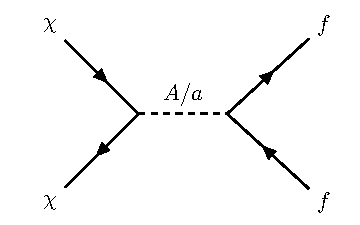
\includegraphics[width=0.35\textwidth]{texinputs/05_relic/figures/feynman/graph_2hdm_relic_s_fermions.pdf}
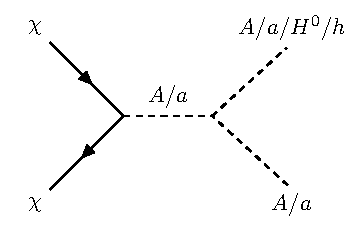
\includegraphics[width=0.35\textwidth]{texinputs/05_relic/figures/feynman/graph_2hdm_relic_s_bosons.pdf}
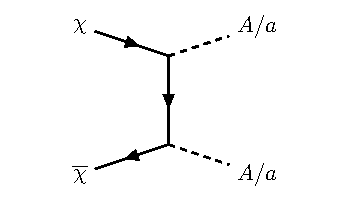
\includegraphics[width=0.35\textwidth]{texinputs/05_relic/figures/feynman/graph_2hdm_relic_ss_bosons.pdf}
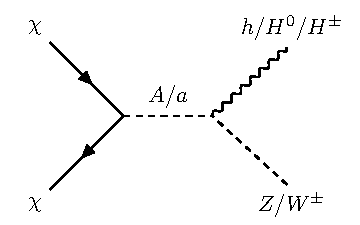
\includegraphics[width=0.35\textwidth]{texinputs/05_relic/figures/feynman/graph_2hdm_relic_s_vbosons.pdf}

\caption{Annihilation diagrams taken into account in the relic density calculation.}
\label{fig:feyn_annihilation}
\end{figure}

The \maddm~\cite{Backovic:2013dpa,Backovic:2015cra} plugin for \mgamcnlo is used to calculate the present-day relic density for this model.
%By modeling the thermal evolution of the cross-section during the expansion of the early universe, the time of freeze-out is determined.
All tree-level annihilation processes are taken into account, and the Yukawa couplings of all fermions are taken to be non-zero.
The Feynman diagrams of annihilation processes taken into account in this calculation are shown in \autoref{fig:feyn_annihilation}. Generally, the annihilation proceeds via single or double s-channel exchange of the pseudoscalars $a$ and $A$, with subsequent decays. Since \maddm uses only tree-level diagrams, contributions from off-shell pseudoscalars can only be taken into account for the case of single s-channel mediation with direct decay of the pseudoscalars to SM fermions. If the pseudoscalars instead decays to other bosons or if the annihilation proceeds through double s-channel diagrams, the outgoing bosons are taken to be on-shell and their decays are not simulated. 

Following \autoref{sec:ParameterScan}, we use the parameter choices $sin(\theta)=0.35$, $m_{h} = 125 GeV$, $g_{\chi}=1$, $\lambda_i = 3$ for all scans in this section.

\subsection{Results}

\begin{figure}[h]
\centering
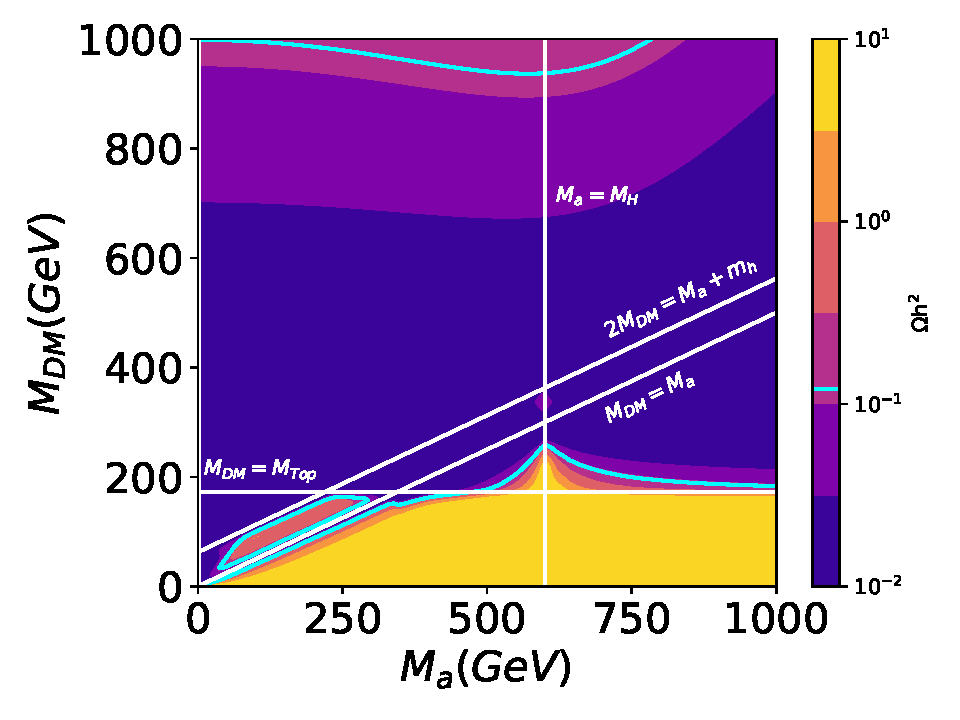
\includegraphics[width=0.49\textwidth]{{texinputs/05_relic/figures/relic/contour_scan_mxd_ma.pdf}}
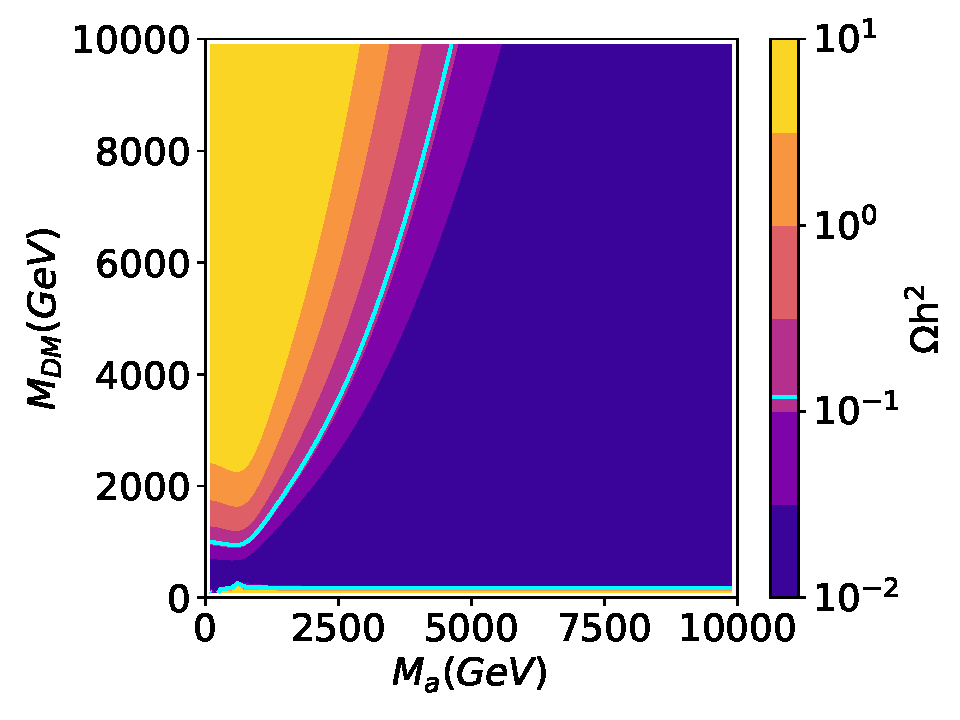
\includegraphics[width=0.49\textwidth]{{texinputs/05_relic/figures/relic/contour_scan_mxd_ma_large.pdf}}
\caption{Predicted relic density for a two-dimensional scan of \mDM and \ma. The other parameters of the model remain fixed with $m_{H}=m_{A}=m_{H^{\pm}}=\unit[600]{GeV}$ and $\tanb=1$, as well as the default choices described in the text. The color scale indicates the relic density, the cyan solid line shows the observed value of $\Omega h^{2} = 0.12$. The color scale is truncated at its ends, i.e. values larger than the maximum or smaller than the minimum are shown in the same color as the maximum/minimum. While the left focuses on the mass region relevant to collider searches, the right panel shows the development of the relic density for a larger mass region.}
\label{fig:relic_scan_mxd_ma}
\end{figure}

The relic density is shown for in the \ma-\mDM plane in \autoref{fig:relic_scan_mxd_ma}.
For small values of $\mDM$ below the mass of the top quark, DM is mostly overabundant. 
In this regime, annihilation to quarks is suppressed by the small Yukawa couplings of the light fermions. 
The observed relic density can only be achieved for $\mDM\approx\ma/2$, where annihilation is resonantly enhanced, or for $\mDM \approx (\ma+\mh)/2$, close to the threshold for the $\chi\chi\rightarrow h a$ process.
Above the top threshold, annihilation into fermions becomes very efficient and DM is underabundant. 
As \mDM increases further, annihilation via single s-channel diagrams is increasingly suppressed and the relic density rises again. 
The observed density is produced by this model for $\mDM\approx1 \mathrm{TeV}$ at low \ma.
\textbf{[The following sentence is being checked with Andreas Albert - would remove]} For values of \ma beyond the LHC reach of a few TeV, the allowed parameter region at the top threshold $\mDM\approx m_{\mathrm{top}}$ remains independent of the value of \ma, indicating that a DM candidate that is mass degenerate with the top quark cannot be excluded by LHC searches alone.

\begin{figure}[h]
\centering
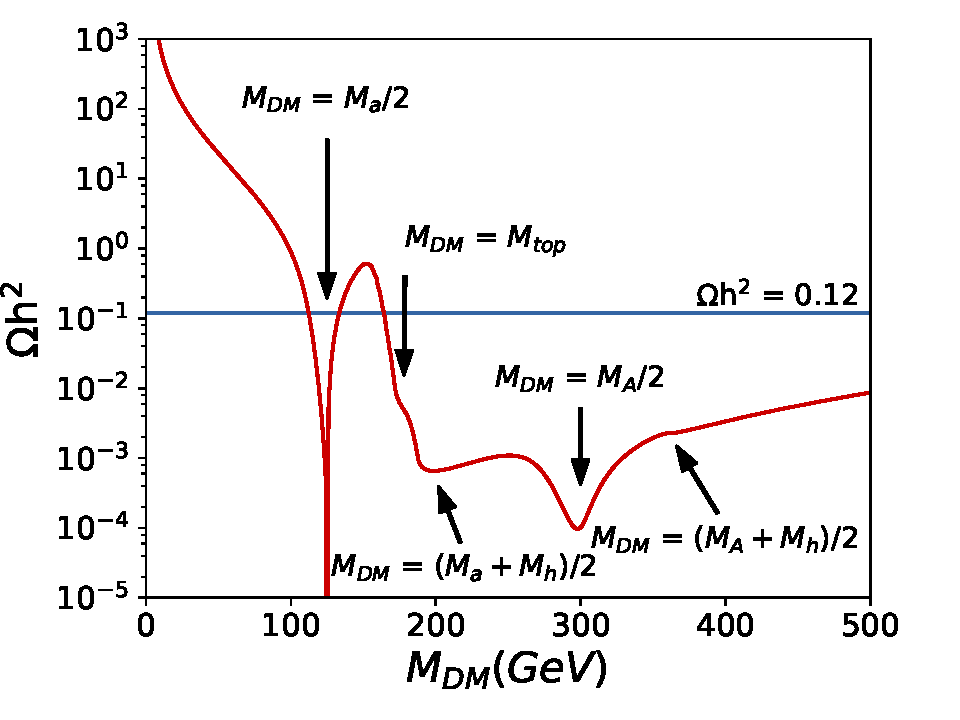
\includegraphics[width=0.8\textwidth]{texinputs/05_relic/figures/relic/line_scan_mdm.pdf}
\caption{Relic density for a one-dimensional scan of \mDM. The other parameters of the model remain fixed with $m_{H}=m_{A}=m_{H^{\pm}}=\unit[600]{GeV}$, $\ma=\unit[250]{GeV}$ and $\tanb=1$, as well as the default choices described in the text. Various kinematic thresholds and regions of resonant enhancement are visible. Consistency with the observed value of $\Omega h^{2} = 0.12$ is mainly controlled by the resonant enhancement of $\chi\chi\rightarrow a$, as well as the onset of $\chi\chi\rightarrow t\overline{t}$.}
\label{fig:relic_scan_mxd}
\end{figure}

The dependence of the relic density on the choice of \mDM is further explored by performing a one-dimensional scan as a function of the DM mass fixing \mH = \mA = $m_{H^{\pm}}$ = 600GeV, \ma = 250GeV, and shown in \autoref{fig:relic_scan_mxd}. 
The relic density confirms structures corresponding to the previously discussed regions of resonant enhancement and to the kinematic boundaries. 
Overall, the behavior is dominated by the low-\mDM suppression of the annihilation cross-section, the resonant enhancement at $\mDM = \ma/2$ and the kinematic top thresholds. 
Other effects, such as the resonant enhancement of $\chi\chi\rightarrow A$ annihilation are present, but only have small effects. 

\begin{figure}[h]
\centering
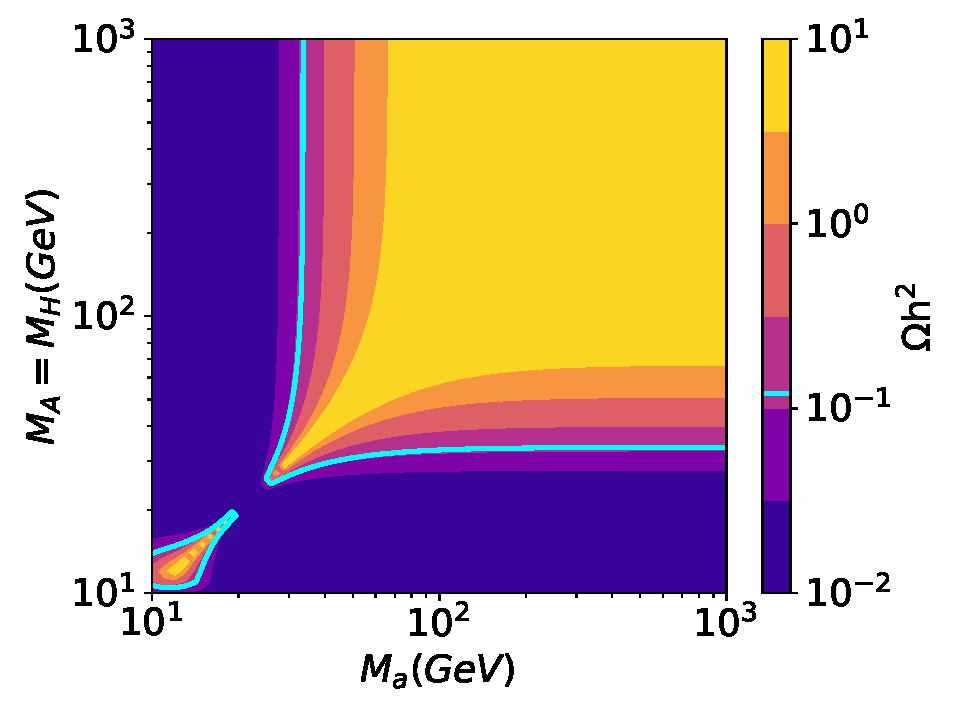
\includegraphics[width=0.49\textwidth]{{texinputs/05_relic/figures/relic/contour_scan_mA_ma_mxd10.pdf}}
\caption{Predicted relic density for a two-dimensional scan of \ma and $\mA=\mH=\mHc$. The other parameters of the model remain fixed with $\mDM=\unit[10]{GeV}$, $\tanb=1$, \mH = \mA = $m_{H^{\pm}}$. The color coding is identical to Fig.~\ref{fig:relic_scan_mxd_ma}.}
\label{fig:relic_scan_mA_ma}
\end{figure}

The relic density values for the \ma-\mA/\mH scan described in \autoref{sec:ParameterScan} is shown in \autoref{fig:relic_scan_mA_ma}. 
For the model parameters chosen in this whitepaper, the regions where the model generates a relic density compatible with the measured value are located at relatively small values of $\ma < \unit[30]{GeV}$ or $\mA=\mH=\mHc < \unit[30]{GeV}$, which are already excluded by LHC and LEP searches (see section 4 of Ref.~\cite{Bauer:2017ota}). 
The cosmological production of DM is largely driven by the choice of $\mDM$. As shown in \autoref{subsub:mDMKinematics}, the model kinematics is largely insensitive to this choice if $\mDM < 2 \ma$. Future experimental results that are sensitive to DM masses around 100 GeV which can yield the measured relic density can still be interpreted by rescaling samples generated according to this parameter scan. 

The $\tanb$-dependent scans, as a function of \ma and \mDM, are shown in Fig.~\ref{fig:relic_scan_mass_tanbeta}. The choice of \tanb acts as an overall modifier of the annihilation cross-section and thus the relic density, and the effect is largely independent of the choice of $\ma$ and $\mDM$. For a choice of $\tanb\approx0.6$, the relic density becomes maximal and steadily decreases for larger and smaller values of \tanb. In the $\mDM$ dependent scan, where \ma is fixed to 250 GeV, the reduction of the relic density at low ($\approx0.1$) and high ($\approx3$) values of $\tanb$ leads to the disappearance of the overabundant island around $\mDM\approx\ma/2$.

\begin{figure}[h]
\centering
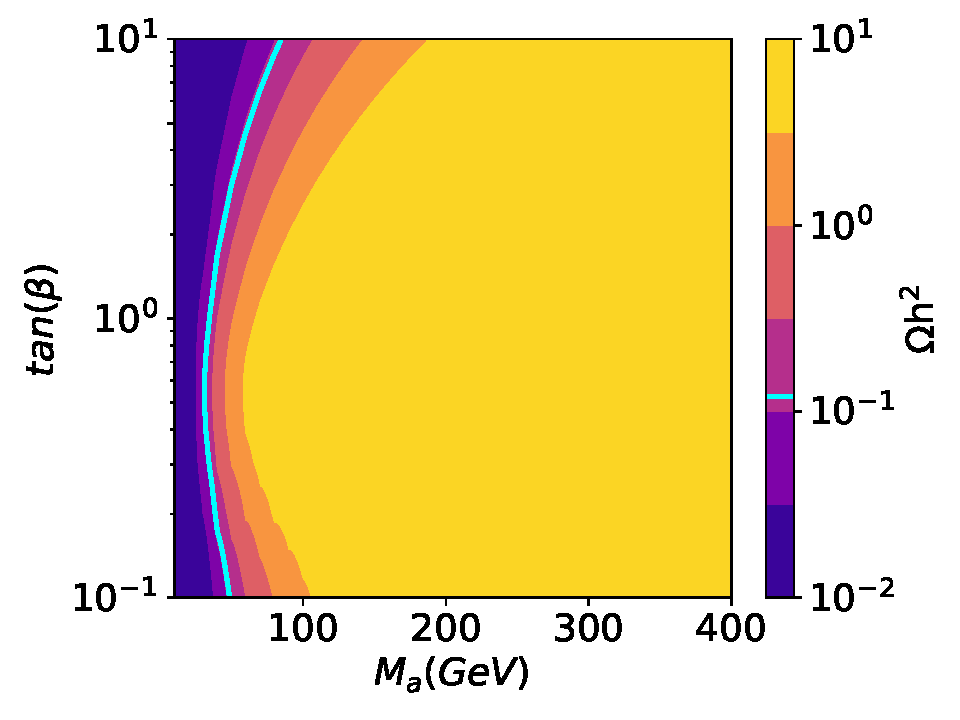
\includegraphics[width=0.49\textwidth]{{texinputs/05_relic/figures/relic/contour_scan_ma_tanbeta.pdf}}
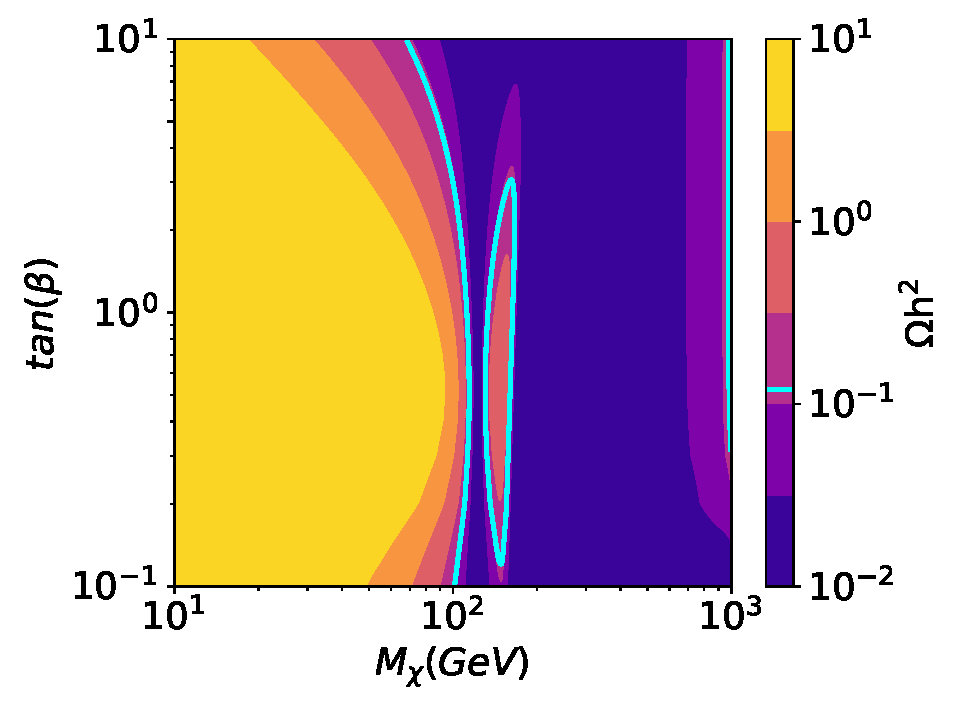
\includegraphics[width=0.49\textwidth]{{texinputs/05_relic/figures/relic/contour_scan_mxd_tanbeta.pdf}}
\caption{Predicted relic density for a two-dimensional scan of \tanb and \ma (left), \mDM (right). In the case of the \mDM ($\ma$) dependent scan, $\ma=\unit[250]{GeV}$ ($\mDM=\unit[10]{GeV}$) is used. The other parameters of the model remain fixed with $m_{H}=m_{A}=m_{H^{\pm}}=\unit[600]{GeV}$, as well as the default choices described in the text. The color coding is identical to Fig.~\ref{fig:relic_scan_mxd_ma}.}
\label{fig:relic_scan_mass_tanbeta}
\end{figure}

%\subsection{Scalar}
%
%\begin{figure}
%    \centering
%    \hspace{2em} 
%    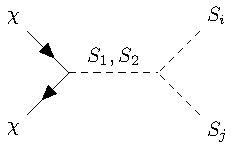
\includegraphics{texinputs/05_relic/figures/relic_scalar/XXSS.pdf} \hspace{3em} \vspace{2em} 
%    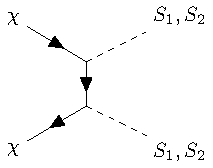
\includegraphics{texinputs/05_relic/figures/relic_scalar/XXSSt.pdf} \hspace{3em} 
%    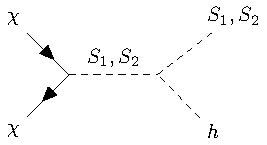
\includegraphics{texinputs/05_relic/figures/relic_scalar/XXSh.pdf}  \hspace{0.5em} \\ 
%    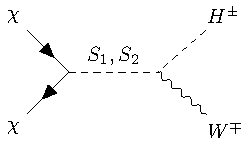
\includegraphics{texinputs/05_relic/figures/relic_scalar/XXWH.pdf} \hspace{2em} 
%    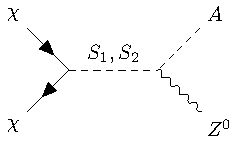
\includegraphics{texinputs/05_relic/figures/relic_scalar/XXZA.pdf} \hspace{2em} 
%    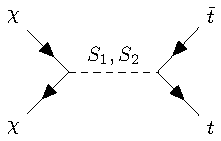
\includegraphics{texinputs/05_relic/figures/relic_scalar/XXtt.pdf} 
%    \caption{Dominant DM annihilation channels, where $(S_i,S_j)$ is one of these scalar final states: $(S_1,S_1)$, $ (S_1,S_2)$, $(S_2,S_2)$, $(H^+,H^-)$, $(A,A)$.}
%    \label{fig:feyn}
%\end{figure}
%
%The 2HDM+S scenario has multiple DM annihilation channels.
%There are tree-level annihilations to fermion-antifermion pairs,
%scalars (the SM Higgs, the two neutral scalars, the pseudoscalar, and the
%charged scalars) and/or the electroweak gauge bosons,
%namely: $\overline{\chi}\chi \rightarrow \overline{f}f$, $S_1 S_1$, $S_2
%S_2$, $S_1 S_2$, $H^+ H^-$, $H^+ W^-$, $A A$, $A Z$, $S_1 h$, and $S_2
%h$ -- these are shown in Fig.~\ref{fig:feyn}. This is to be compared with a single mediator model in which only
%the $\overline{f}f$ and $SS$ channels are present. Note that since all
%diagrams involve $\chi$-scalar vertices (including those with gauge
%boson final states) they are all $p$-wave processes. As such, while we
%will easily be able to find parameters that accommodate the observed
%relic density, there will be no constraints arising from indirect
%detection because the $p$-wave annihilation processes are highly velocity
%suppressed in the late universe.
%
%
%If the DM particle is relatively light, such that annihilation to the
%scalars and electroweak bosons is kinematically forbidden ($m_\chi \lesssim
%80\GeV$), the only annihilation channels that remain open are the
%fermionic ones.  This case is heavily constrained, as the dominant
%annihilation channel is then $b\bar{b}$, which is suppressed by the
%bottom Yukawa coupling and thus usually requires resonant enhancement
%to accommodate the correct relic density.
%
%
%If, instead, the DM particle is heavy enough to annihilate to the Higgs,
%electroweak gauge bosons and/or the new scalars, then these final states will
%likely dominate due to the Yukawa suppression of annihilations to fermions 
%(top excluded).
%Because all of these annihilations are governed by scalar and electroweak
%couplings -- and exist due to gauge invariance, independent of the
%Yukawa couplings of the second doublet -- they are also present,
%for example, in the limit where the second doublet is inert.
%This ability to produce the correct relic abundance independent of
%Yukawa structure means that DM can be adequately produced while
%avoiding any Yukawa dependent constraints (e.g. DD, neutral meson
%mixing, $b \to s \gamma$, $\mu \to e \gamma$, etc.).
%
%%%%%%%%%%%%%%%%%%%%%%%%%%%%%%%%%%%%%%%%%%%
%\begin{figure}[t]
%\centering
%\begin{subfigure}[t]{0.43\textwidth}
%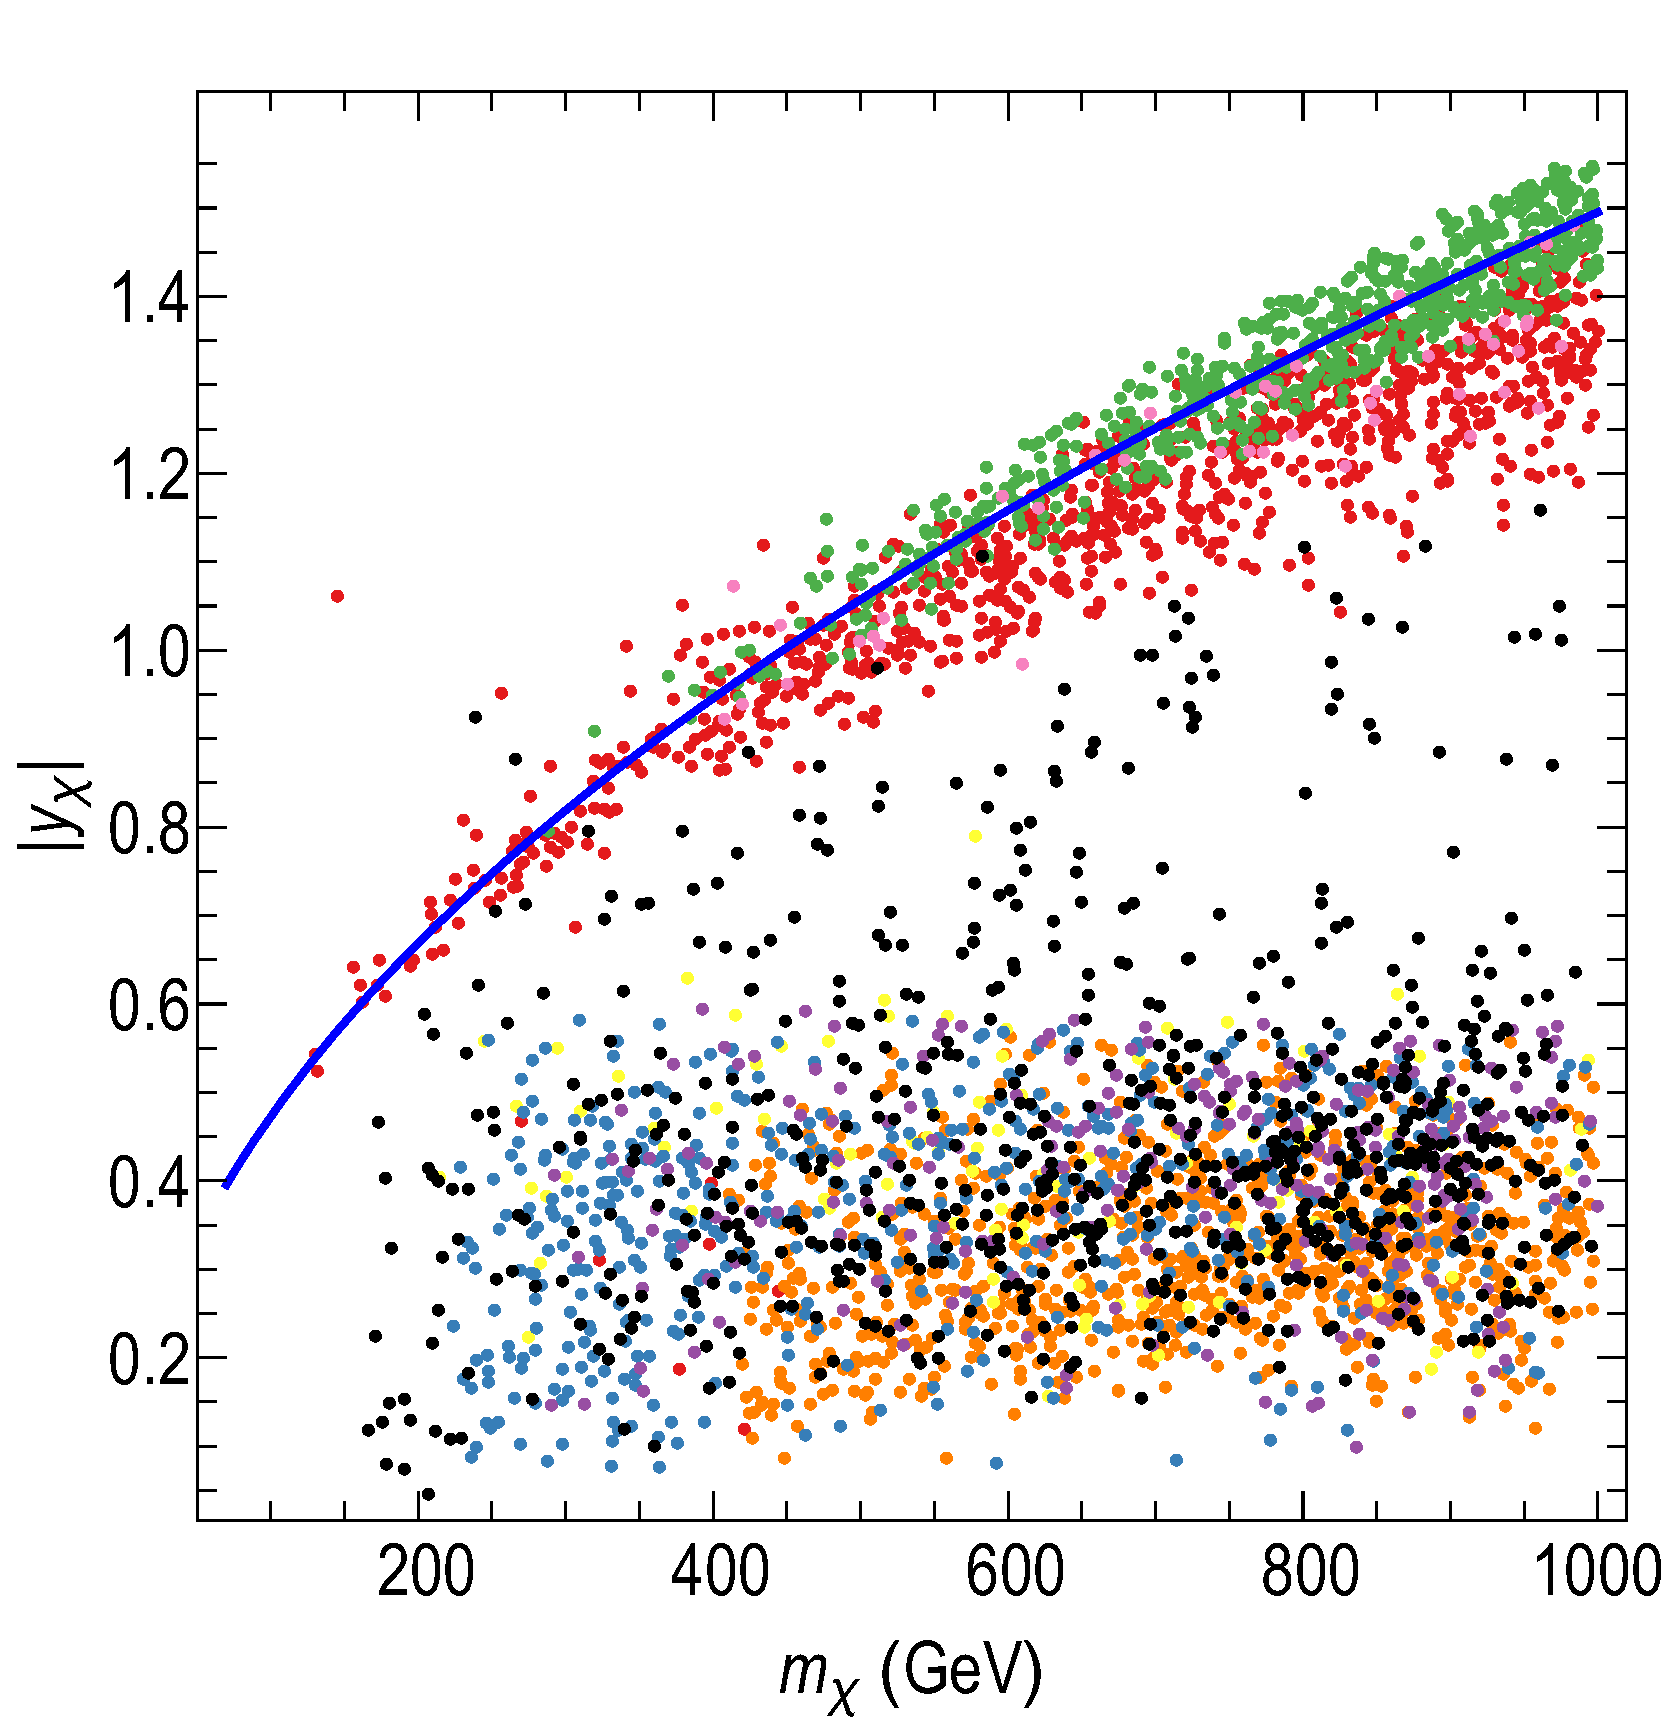
\includegraphics[width=\textwidth]{texinputs/05_relic/figures/relic_scalar/mDM_yDM4.pdf}
%\label{fig:scan1a}
%\end{subfigure}
%\hspace{1em}
%\begin{subfigure}[t]{0.43\textwidth}
%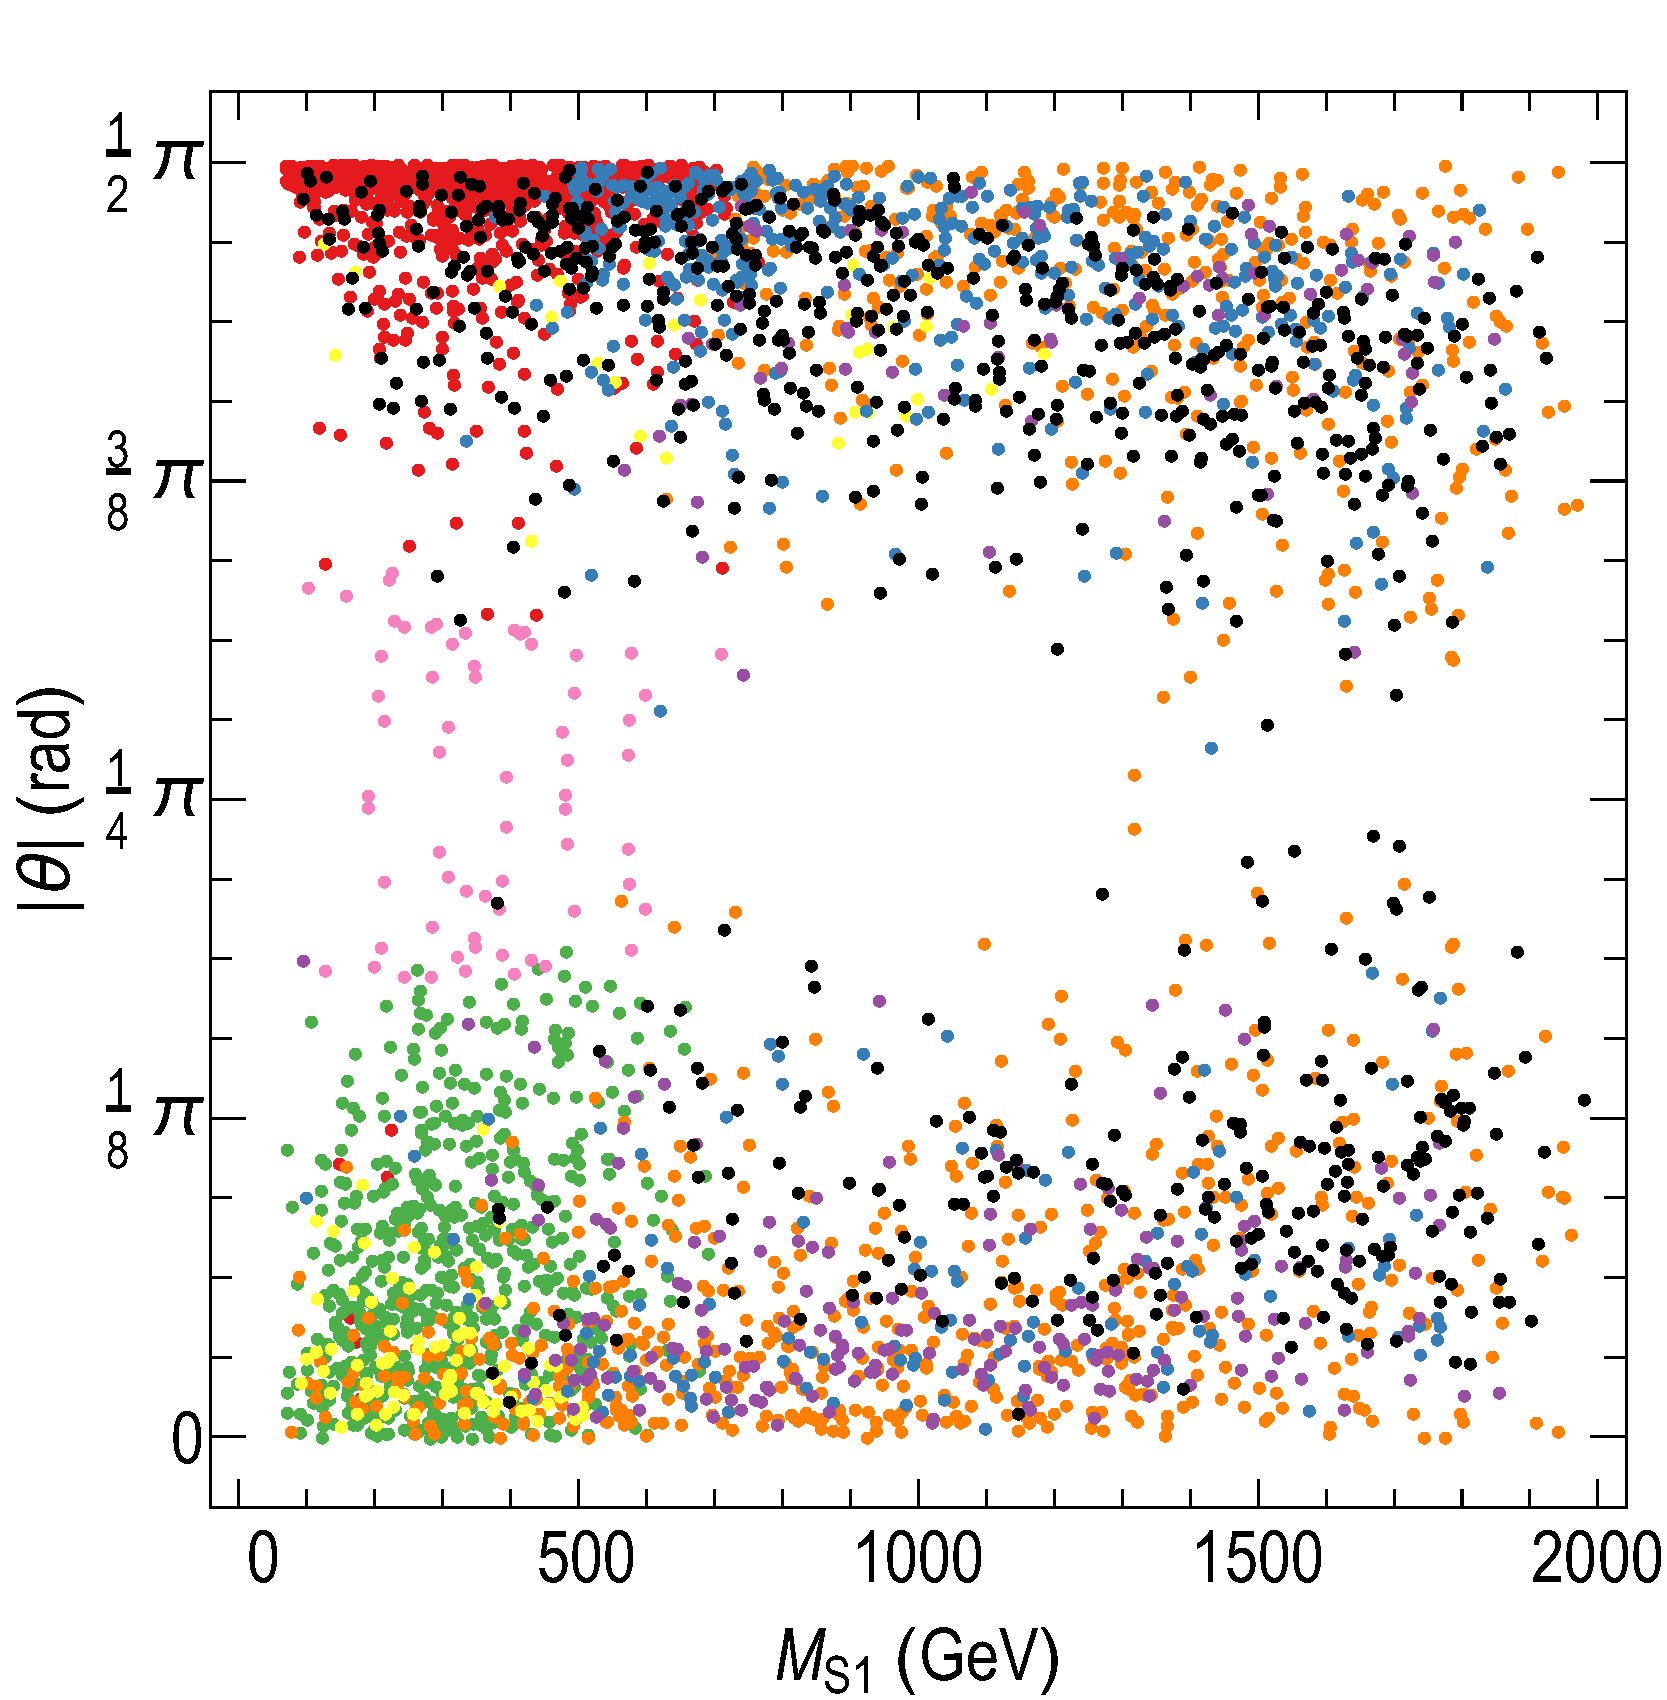
\includegraphics[width=\textwidth]{texinputs/05_relic/figures/relic_scalar/MS1_Theta2.pdf}
%\label{fig:scan1b}
%%\caption{\centering Second Higgs and scalar singlet mixing angle versus DM mass. The plot is symmetric across $| \theta | = \pi / 2$ if extended.}
%\end{subfigure}
%\vspace{0.5ex}
%\begin{subfigure}[t]{0.43\textwidth}
%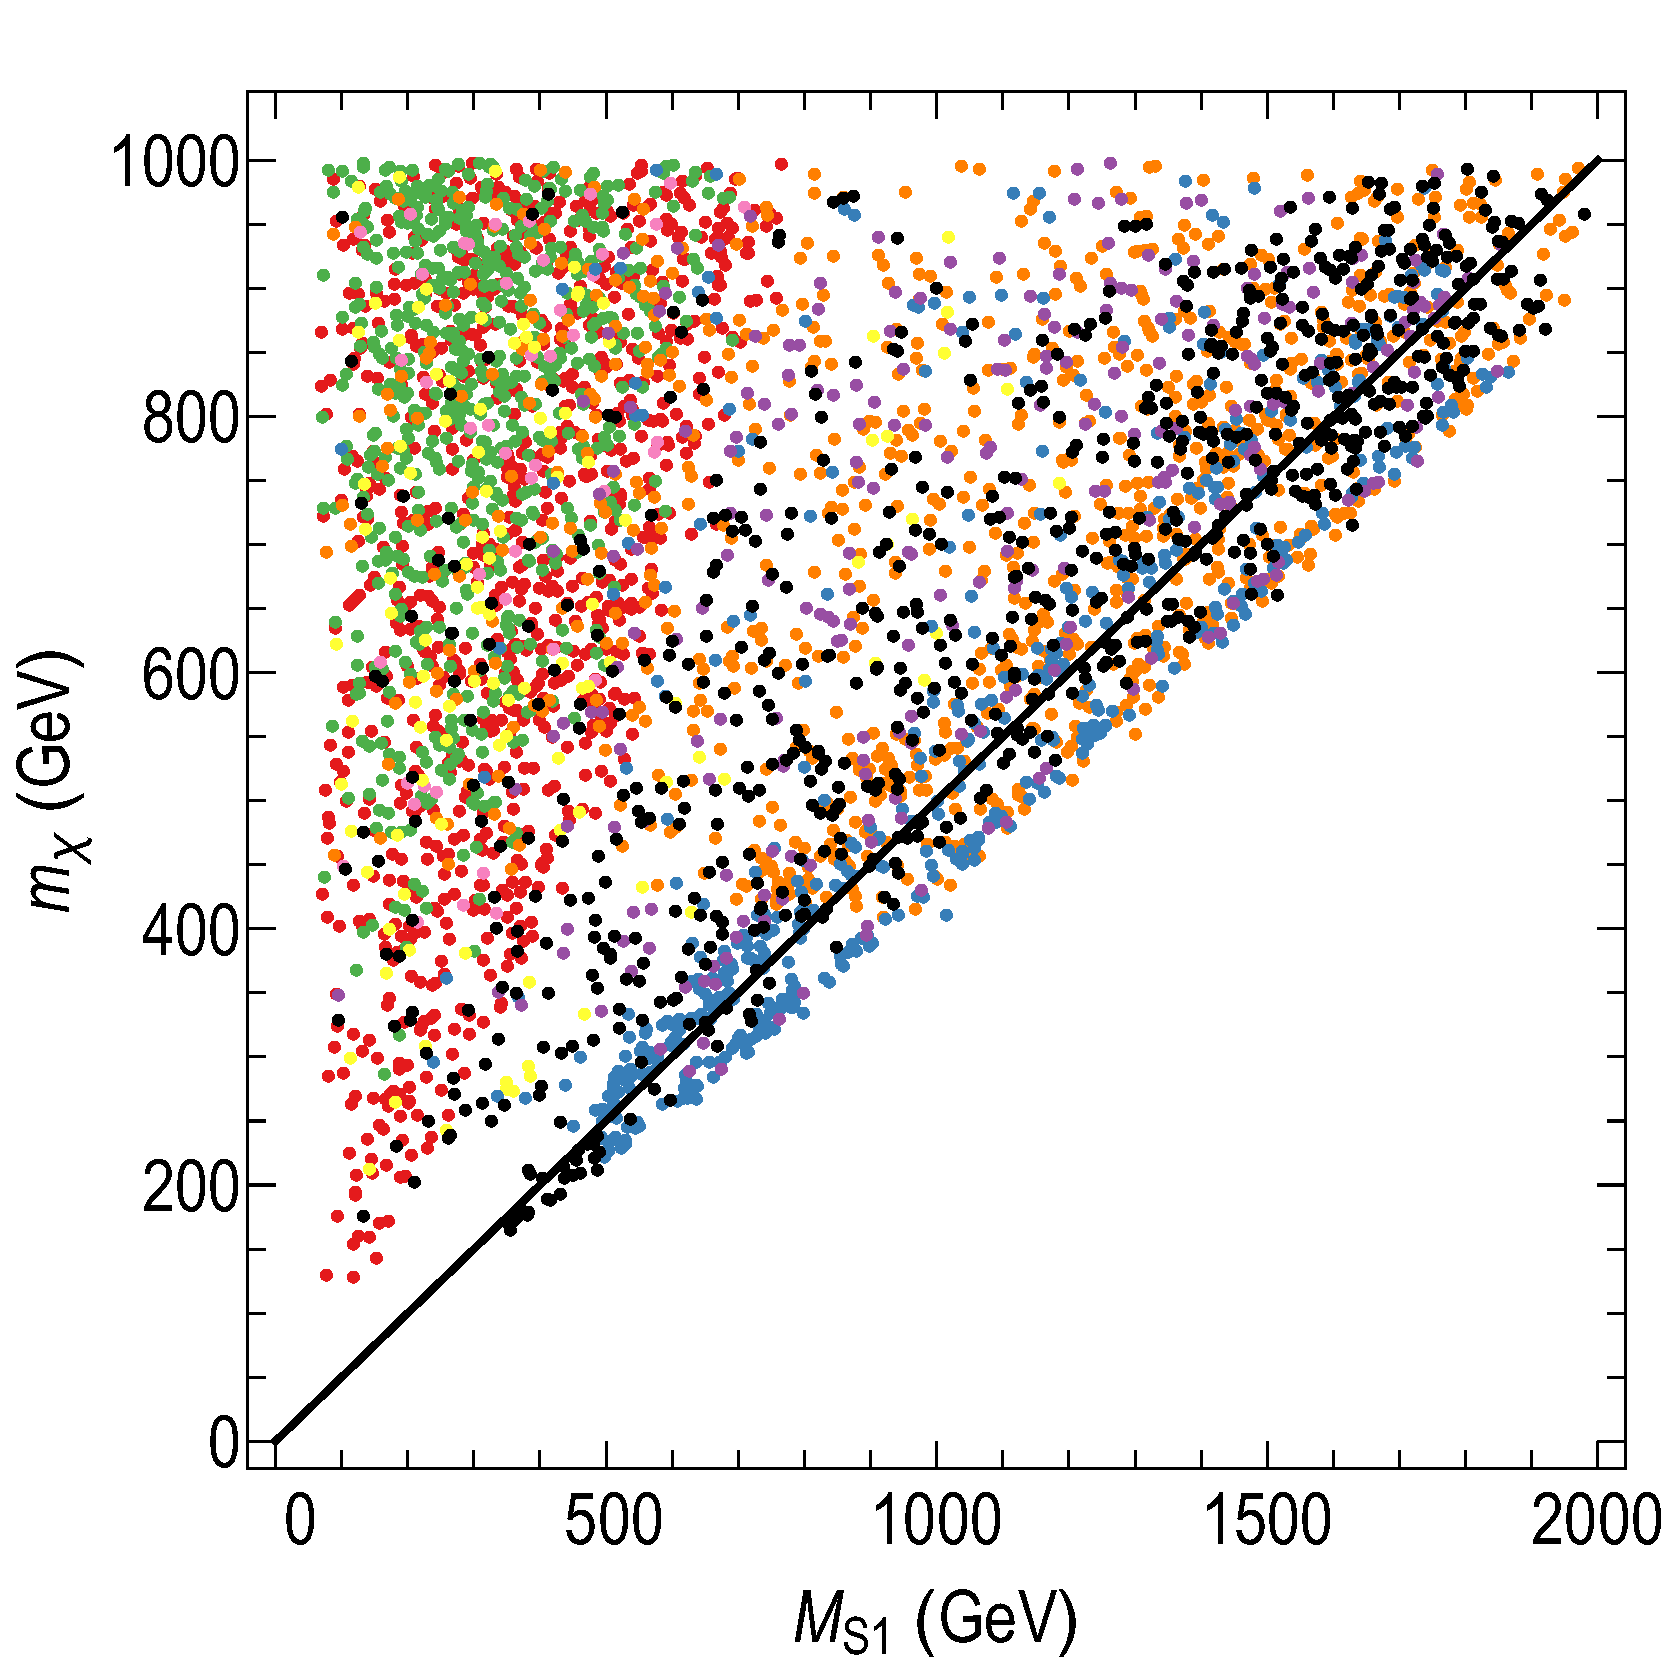
\includegraphics[width=\textwidth]{texinputs/05_relic/figures/relic_scalar/MS1_mDM3.pdf}
%%\caption{DM mass - lighter scalar mass plane $m_\chi - M_{S_1}$.}
%\label{fig:scan1c}
%%\caption{\centering Two additional neutral scalar masses. Note that we have chosen $M_{S_2} > M_{S_1}$; if this is relaxed, then the plot is simply symmetric across the solid black line.}
%\end{subfigure}
%\hspace{1em}
%\begin{subfigure}[t]{0.43\textwidth}
%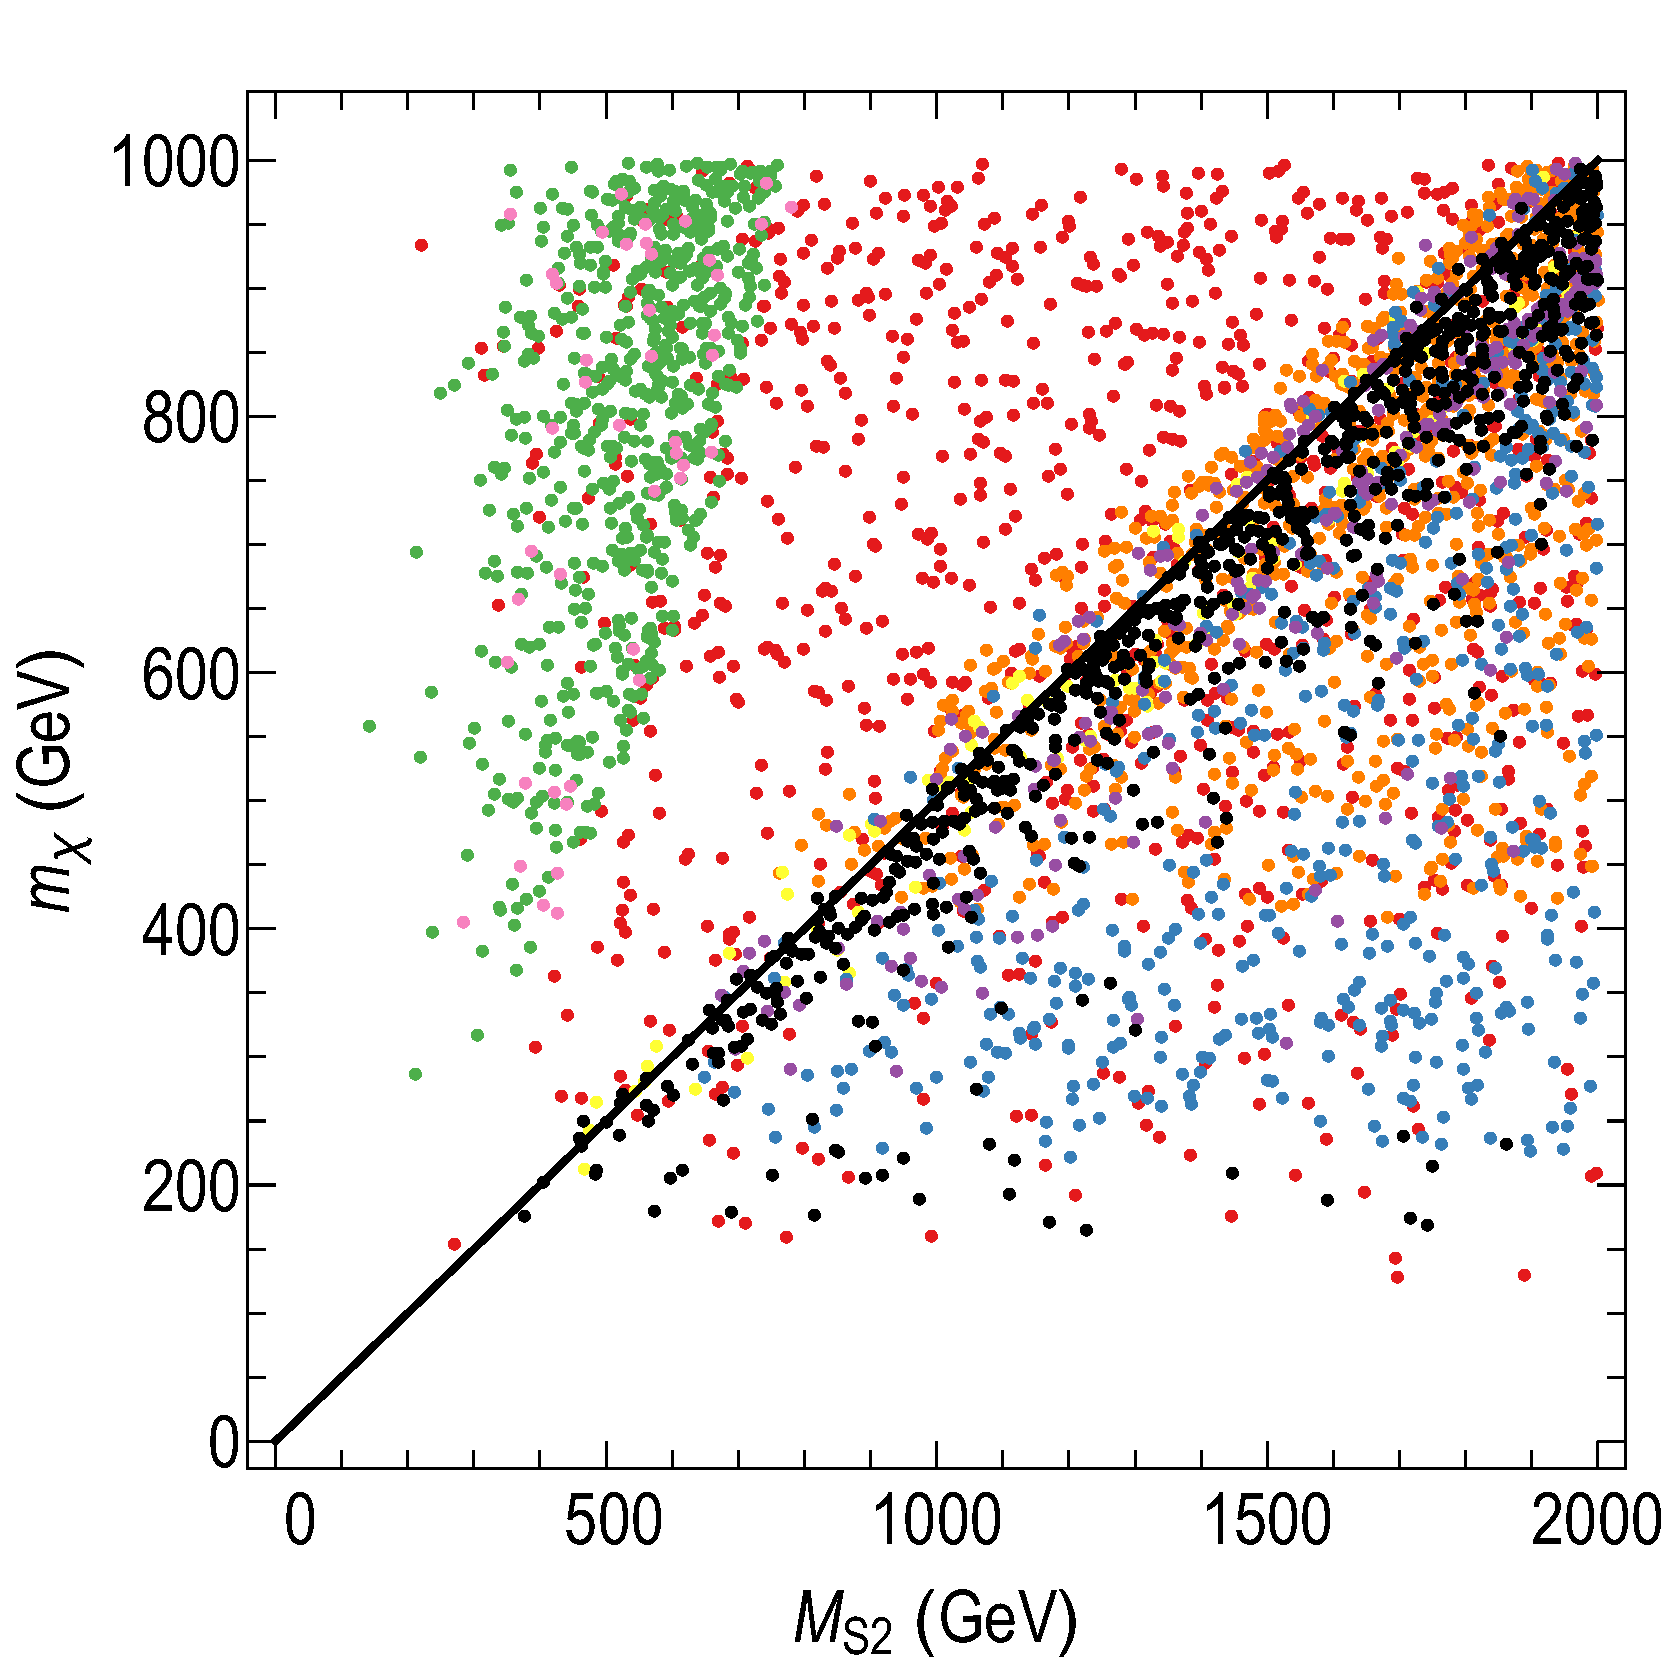
\includegraphics[width=\textwidth]{texinputs/05_relic/figures/relic_scalar/MS2_mDM3.pdf}
%%\caption{DM mass - heavier scalar mass plane $m_\chi - M_{S_2}$.}
%\label{fig:scan1d}
%%\caption{\centering DM mass versus lightest new scalar mass eigenstate.}
%\end{subfigure}\\
%\begin{subfigure}[t]{0.86\textwidth}
%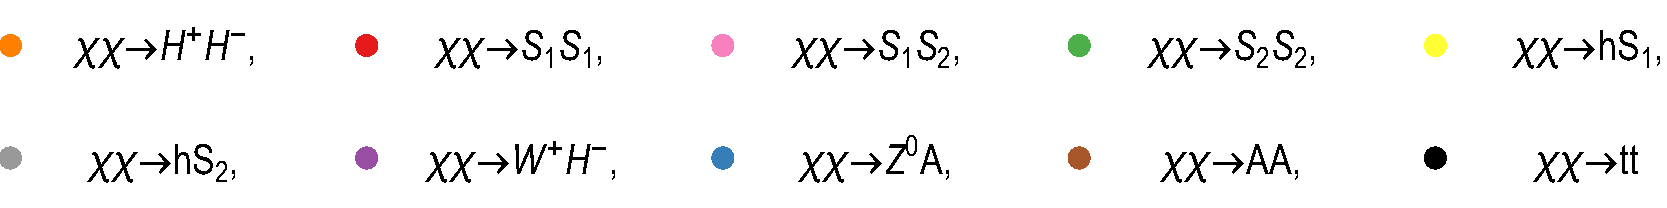
\includegraphics[width=\textwidth]{texinputs/05_relic/figures/relic_scalar/LegendH2.pdf}
%\end{subfigure}
%\caption{Points of our scan of parameter space that produce the correct relic density. The colours represent the dominant annihilation channel, as shown above. 15000 points are taken that survive the constraints, and of them only 25\% of the $H^+H^-$ channel and 10\% of the $S_1S_1$ channel are shown for clarity. The black line in the lower panels indicate $m_\chi = 2 M_{S_1, S_2}$, which is the resonance condition for the s-channel annihilation processes. The blue line in the top left panel represents the scaling expected for a cross section of $\langle \sigma v \rangle \sim y^4_\chi v^2 / 16 \pi^4 m_\chi^2$ which, in this model, applies to a pure $\overline{\chi}\chi \to S_iS_i$ scenario.}
%\label{fig:scan1}
%\end{figure}
%%%%%%%%%%%%%%%%%%%%%%%%%%%%%%%%%%%%%%%%%%%
%
%We implemented the model in Feynrules\footnote{The Feynrules model file used is publicly available in the Feynrules model database.} \citep{Christensen:2008py,Alloul:2013bka} and output the model with the CALCHEP interface~\citep{Christensen:2009jx}. We then used {\tt micrOMEGAs}~\citep{Barducci:2016pcb} to perform the relic density calculation, where we included 3 body final states with off-shell gauge bosons. We also double checked the results by calculating the annihilation cross sections, which are reported in \citep{Bell:2017rgi}. In the case where the parameter values are away from resonances and annihilation thresholds, one can use the wave expansion of the cross sections. The p-wave coefficients of this expansion are also reported in \citep{Bell:2017rgi}.
%
%Sommerfeld enhancement can significantly increase the DM annihilation
%cross section~\citep{Feng:2010zp,Cassel:2009wt,Iengo:2009ni}, provided
%at least one of the scalars is both sufficiently light compared to the
%DM, and strongly coupled to the DM particle.  In practice, for the
%parameter range we consider, this leads to $\mathcal{O}(1)$
%corrections to the cross section; a discussion is provided in
%\citep{Bell:2017rgi}.
%
%%%%%%%%%%%%%%%%%%%%%%%%%%%%%%%%%%%%%%%%%%%
%\begin{figure}[ht]
%\centering
%\begin{subfigure}[t]{0.45\textwidth}
%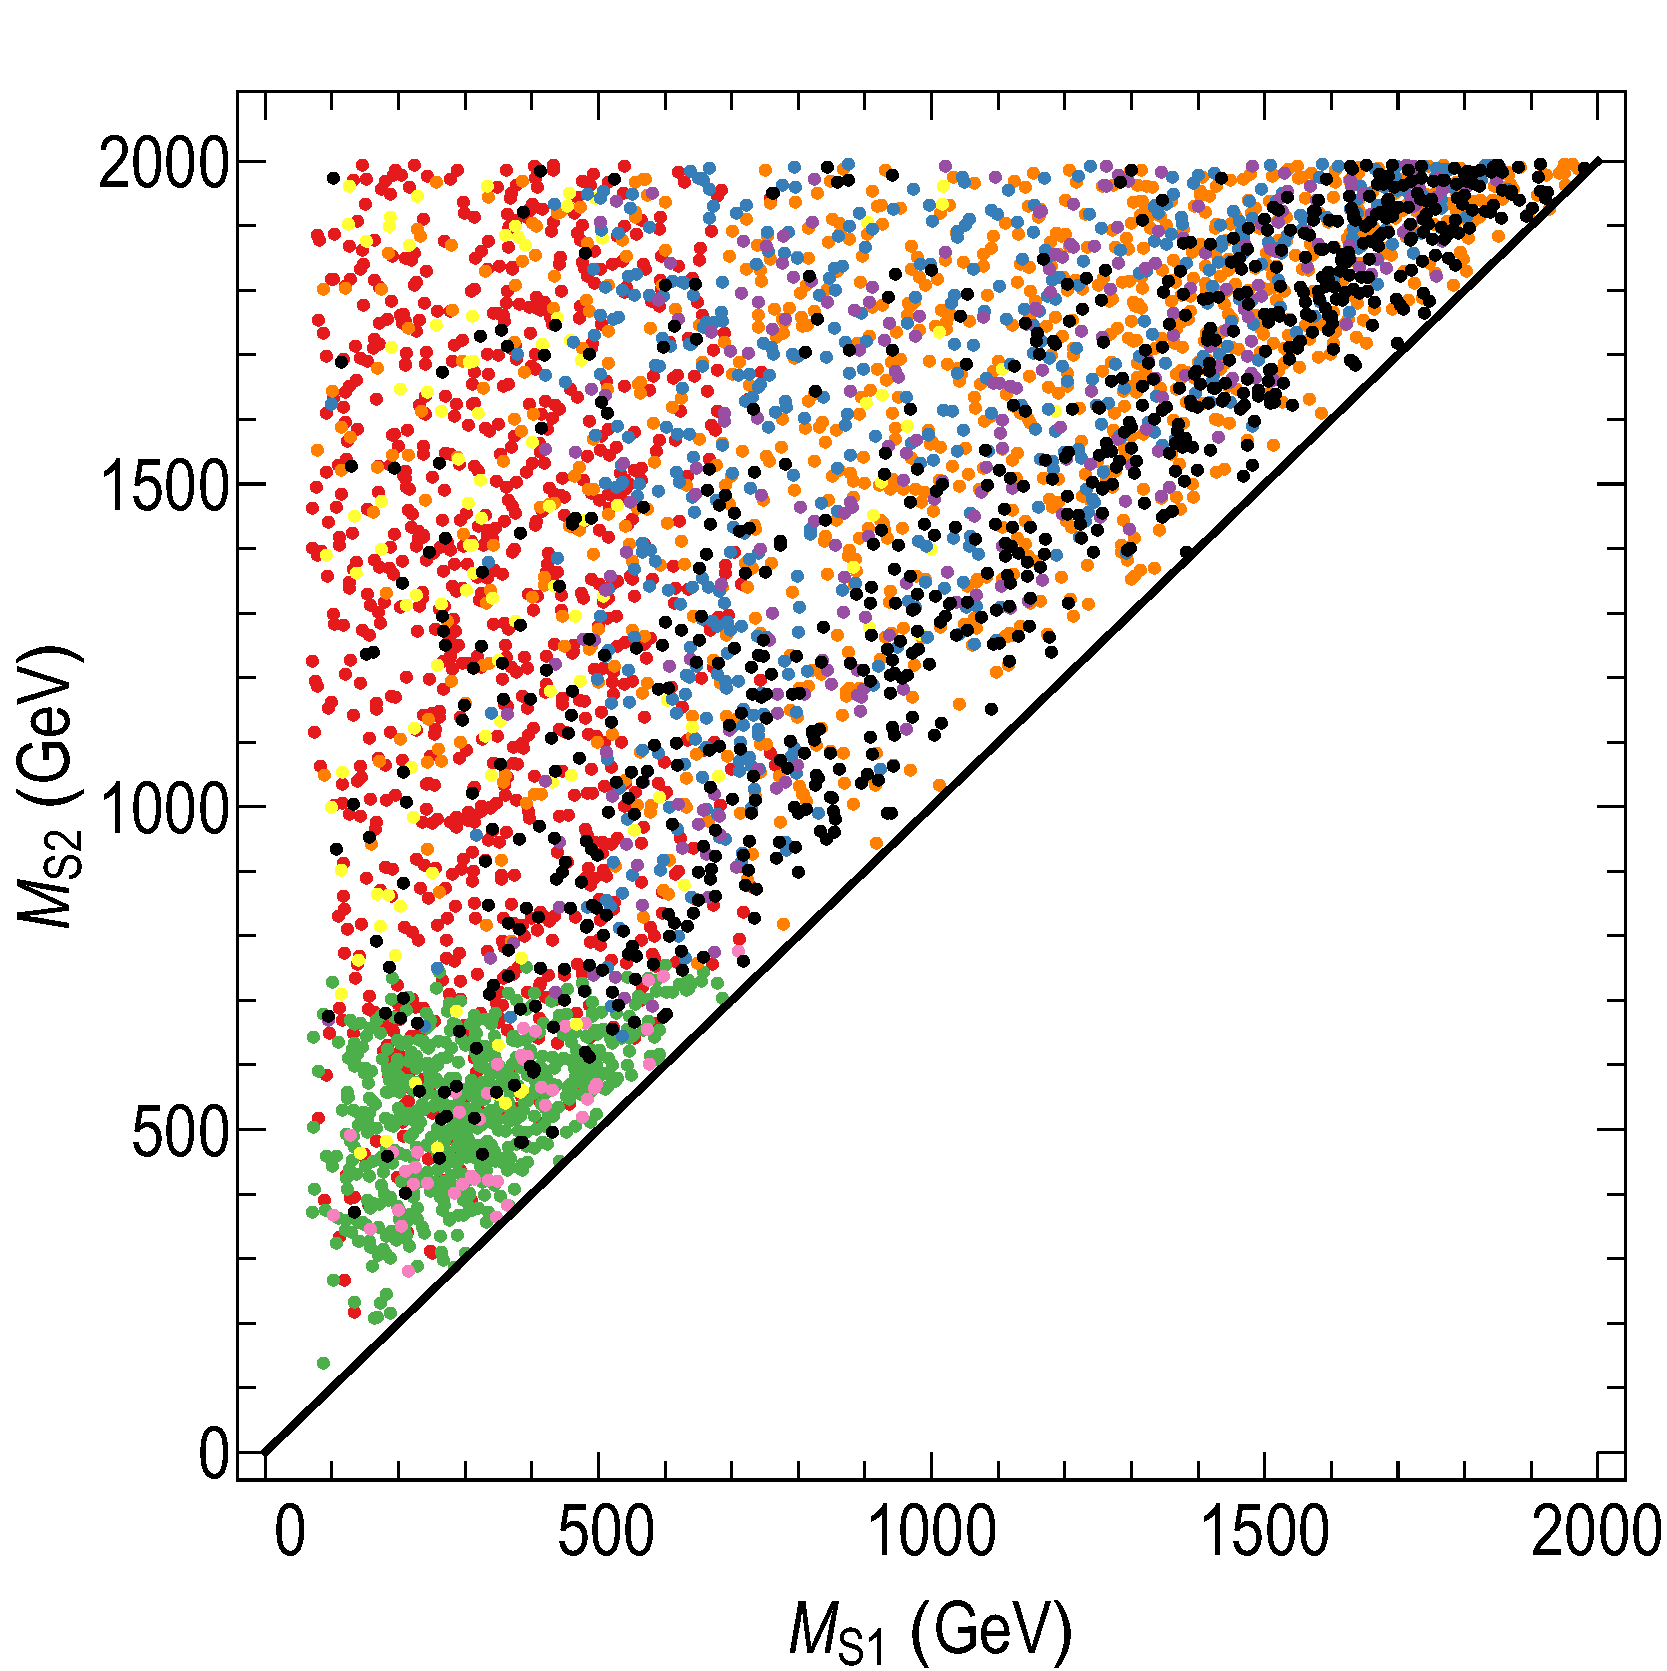
\includegraphics[width=\textwidth]{texinputs/05_relic/figures/relic_scalar/MS1_MS25.pdf}
%%\caption{Heavier - lighter scalar mass plane $M_{S_2} - M_{S_1}$.}
%\label{fig:scan1e}
%%\caption{\centering DM mass versus lightest new scalar mass eigenstate.}
%\end{subfigure}
%\hspace{1em}
%\begin{subfigure}[t]{0.45\textwidth}
%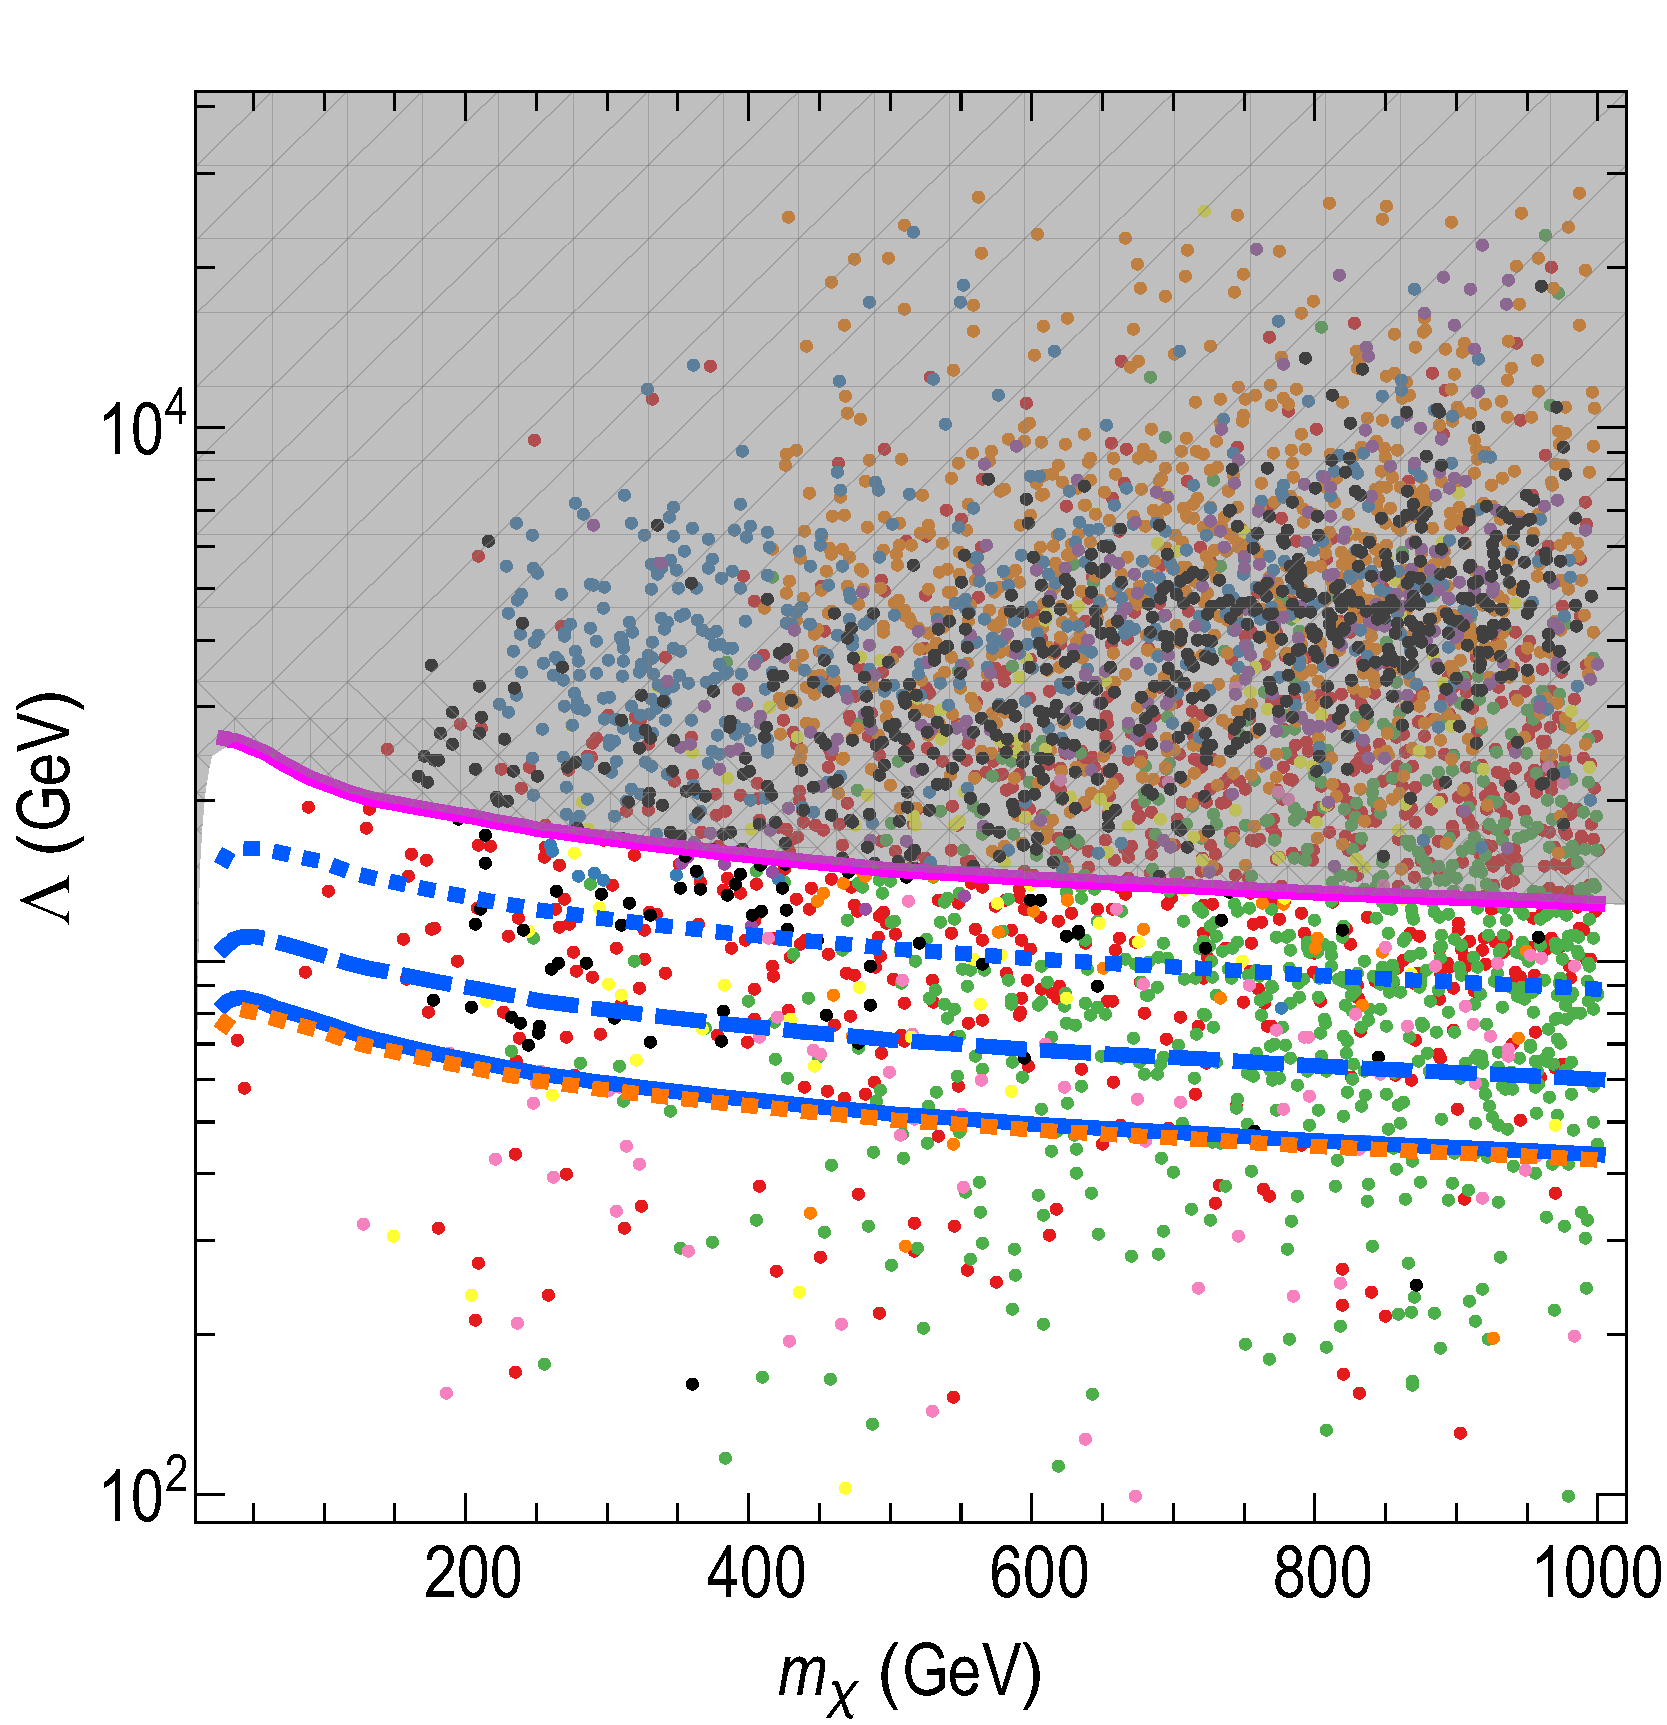
\includegraphics[width=\textwidth]{texinputs/05_relic/figures/relic_scalar/mDM_Lambda4.pdf}
%%\caption{$\Lambda$ versus $m_\chi$}
%\label{fig:scan1f}
%%\caption{\centering DM mass versus lightest new scalar mass eigenstate.}
%\end{subfigure}
%\begin{subfigure}[t]{0.9\textwidth}
%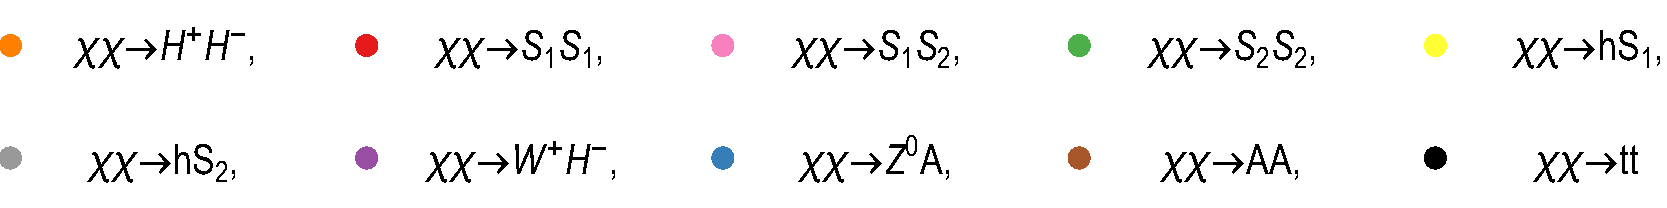
\includegraphics[width=\textwidth]{texinputs/05_relic/figures/relic_scalar/LegendH2.pdf}
%\end{subfigure}
%\caption{Points of our scan of parameter space that produce the correct relic density. The colours represent the dominant annihilation channel, as shown above. 15000 points are taken that survive the constraints, and of them only 25\% of the $H^+H^-$ channel and 10\% of the $S_1S_1$ channel are shown for clarity. $\Lambda$ is the effective cut-off scale for the DD effective operator; the dotted orange line represents the constraint from the LUX 2016 results \citep{Akerib:2016vxi}, the solid blue represents the XENON1T experiment \citep{Aprile:2017iyp}, the dashed blue the projection for the XENON1T experiment with $2t\cdot y$ of data taking, the dotted blue the projection for the XENONnT experiment with $20t\cdot y$ of data taking \citep{Aprile:2015uzo}, and the magenta is the DD sensitivity at the ``neutrino floor''\citep{Billard:2013qya}.}
%\label{fig:scan11}
%\end{figure}
%
%The independent parameters present in the model are
%\be
%m_\chi, \quad M_{S_1}, \quad M_{S_2}, \quad y_\chi, \quad \hat{\lambda}_4, \quad \hat{\lambda}_5, \quad \hat{\lambda}_{hHS}, \quad \hat{\lambda}_{HHS}, \quad \epsilon_u \quad \textrm{and} \quad \epsilon_d.
%\ee
%This set of parameters, through the minima condition and the diagonalization relations, together with the additional constraint $m_\chi = y_\chi v_s$, determine all other parameters of the model\footnote{The phase of the DM Yukawa can always be reabsorbed, so one can chose $y_\chi$ and $v_s$ to be both real and positive.}.
%%
%The scan is performed in the following range:
%\bea
%70\GeV < &m_\chi& < 1\TeV,\\
%70\GeV < &M_{S_1}& < M_{S_2} < 2 \TeV, \\
%0 < &y_\chi& < 2,\\
%&|\hat{\lambda}_{hHS}|& < 2,\\
%&|\hat{\lambda}_{HHS}|& < 4,\\
%0 < &\epsilon_u& < 1,
%\eea
%while for $\hat{\lambda}_4$ and $\hat{\lambda}_5$ we scan over the region shown in \citep{Bell:2017rgi}. 
%These ranges for the couplings were chosen so that most of the points will satisfy unitarity and perturbativity bounds, which was checked via the scalar scattering matrices as in \citep{Bell:2016ekl}.
%To achieve the right relic density, we will see that it will be in general necessary to have $m_\chi\gtrsim M_{S_1}$, and the inequality is strictly required for DM masses below the top mass, as otherwise all considered annihilation channels are closed. In this low DM mass region, however, one needs to take into account Higgs invisible constraints \citep{Aad:2015pla,Khachatryan:2016whc}: 2-body decays forbid the region $2m_\chi<m_h$ and $2M_{S_1}<m_h$, while considering 3-body decays as well further pushes up the lower bound on $M_{S_1}$ to nearly $100\GeV$. The Higgs invisible decays constraints can only be avoided in the $\theta\rightarrow\pi/2$ limit, but in such case the model approaches a decoupled dark sector which is phenomenologically uninteresting\footnote{Relic density requirement can be satisfied in the limit of a decoupled dark sector, in which dark matter annihilates to light dark scalars. However, there would be no signals in collider or direct detection experiments. Moreover, indirect detection is prevented by the p-wave nature of annihilation to scalars, even if small couplings to the SM are included.}. Taking into account these considerations, we have chosen in our scan a conservative lower bound for the DM mass and for the lightest scalar of $70\GeV$.
%Points are selected if they have a relic density between $0.1 < \Omega h^2 < 0.14$ and satisfy all bounds from flavour, unitarity, perturbativity, tree level vacuum stability, and DD constraints. 
%
%\begin{figure}
%\begin{center}
%%\vspace*{1.5cm} 
%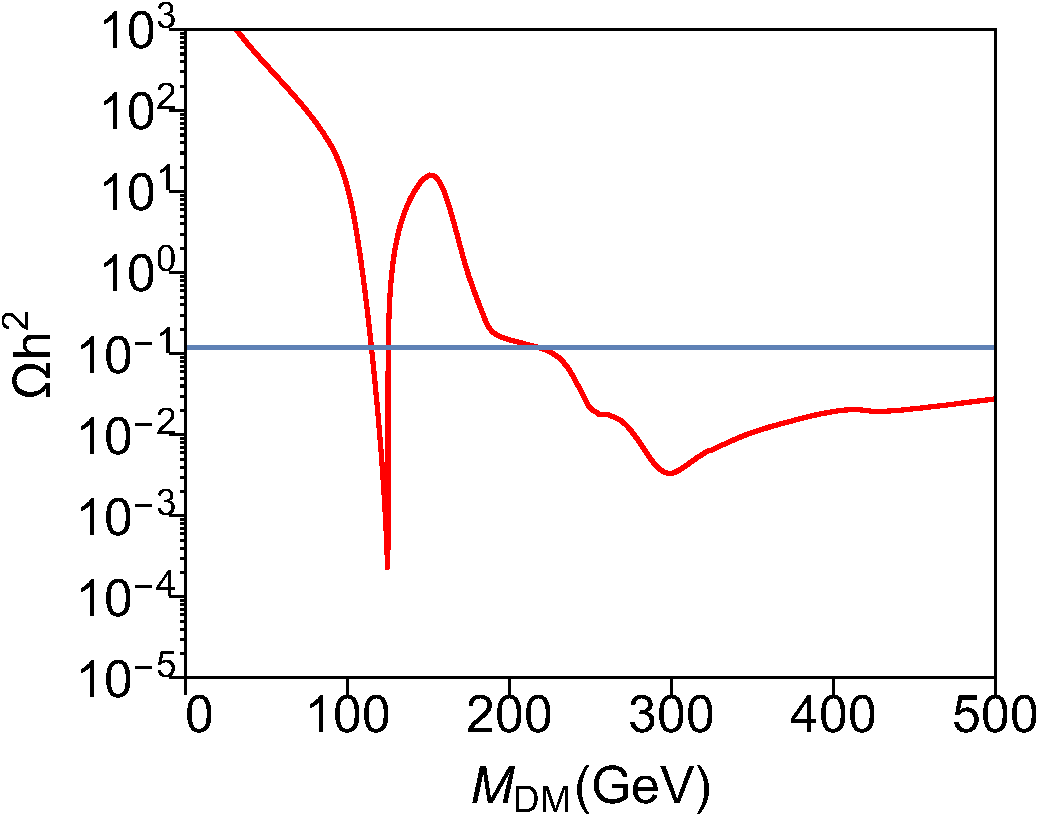
\includegraphics[width=0.7\textwidth]{texinputs/05_relic/figures/relic_scalar/RelicPlot.pdf}
%\caption{One-dimensional scan of the parameter space. We fix all other parameters, see the text for more details.} 
%\label{fig:scalarrelic1D}
%\end{center}
%\end{figure}
%
%The relic density is insensitive to the value of $\epsilon_d$, while the DD results depend on the relationship $\epsilon_d$ and $\epsilon_u$.  
%We set $\epsilon_d = \epsilon_u$ for the scans presented in Fig.~\ref{fig:scan1} and Fig.~\ref{fig:scan11} (with the exception of the right panel of Fig.~\ref{fig:scan11}, which enforces no DD constraint and hence has no $\epsilon_d$ dependence). 
%
%We have chosen to define $S_1$ to be the lighter of the 2 scalars, and allow $\theta$ to range from $0$ to $\pi/2$. As one can always switch the two scalars by sending $\theta\rightarrow\pi/2-\theta$, an equivalent choice would be to take $0<\theta<\pi/4$ without requiring any mass ordering.
%
%In Fig. \ref{fig:scalarrelic1D} we show the value of the relic density obtained through thermal freezeout in a one-dimensional scan, where we kept fixed all parameters except the DM mass. We fix $M_{S_1}=250\GeV$, $M_{S_2}=M_A=M_{H^+}=600\GeV$, $\cos\theta=0.35$ (equivalent to $\sin\theta=0.35$ for the PS model), $y_\chi=1$, 
%
%
%These choices of parameters, along with alignment conditions and $m_\chi = v_s y_\chi$, then fix
%\begin{align}
%    v_s &= \frac{m_\chi}{y_\chi} = m_\chi, \\
%    \lambda_1 &= \frac{m_h^2}{v^2} \sim 0.258, \\
%    \lambda_{s} &= \frac{1}{4 v_s^2} \left( M_{a}^2 + M_A^2 +(M_A^2 - M_a^2) \cos (2\theta ) \right) \sim \frac{222.4^2\GeV^2}{m_\chi^2}, \\
%%    \lambda_{11s} &= 0, \\
%    \lambda_{12s} &= \frac{(M_{S_1}^2 - M_{S_2}^2) \sin (2\theta)}{2 v v_s} \sim -\frac{396.5 \GeV}{m_\chi},\\
%    \lambda_4 &= \frac{1}{2v^2} \left( 2 M_{A}^2 - 4 M_{H^+}^2 + M_{S_1}^2 + M_{S_2}^2 + (M_{S_1}^2 - M_{S_2}^2) \cos (2 \theta ) \right) \sim -0.60, \\
%    \lambda_5 &= -\frac{1}{2v^2} \left( 2 M_{A}^2 - M_{S_1}^2 - M_{S_2}^2 + (M_{S_2}^2 - M_{S_1}^2) \cos (2 \theta ) \right) \sim -0.60, \\
%    \lambda_3 &= \lambda_1 - \lambda_4 - \lambda_5 \sim  1.46.
%\end{align}
%


%%%%%%%%%%%%%%%%

\section{Conclusions}

%\section{Acknowledgements} 
%The work of CD is supported by the European Research Council under the European Union's Horizon 2020 research and innovation programme (ERC grant agreement No. 679305 DARKJETS). UH acknowledges the hospitality and support of the CERN theory division. MF and PT are funded by the European Research Council under the European Union's Horizon 2020 program (ERC grant agreement No. 648680 DARKHORIZONS). AR is supported by the Swiss National Science Foundation (SNSF), project title: `` Investigating the Nature of Dark Matter'', project number: 200020-159223. The work of TMPT is supported in part by National Science Foundation grants PHY-1316792 and PHY-1620638. The work of GL is partially supported by the DOE Award DE-SC0010010.
 

\bibliography{DMWG-2HDM-whitepaper_Main,texinputs/04_grid/DMHF}
\bibliographystyle{JHEP}



\end{document}


